\documentclass{article}

% if you need to pass options to natbib, use, e.g.:
%     \PassOptionsToPackage{numbers, compress}{natbib}
% before loading neurips_2026

% The authors should use one of these tracks.
% Before accepting by the NeurIPS conference, select one of the options below.
% 0. "default" for submission
\usepackage[preprint]{main}
% the "default" option is equal to the "main" option, which is used for the Main Track with double-blind reviewing.
% 1. "main" option is used for the Main Track
%  \usepackage[main]{neurips_2026}
% 2. "position" option is used for the Position Paper Track
%  \usepackage[position]{neurips_2026}
% 3. "eandd" option is used for the Evaluations & Datasets Track
 % \usepackage[eandd]{neurips_2026}
 % if you need to opt-in for a single-blind submission in the E&D track:
 %\usepackage[eandd, nonanonymous]{neurips_2026}
% 4. "creativeai" option is used for the Creative AI Track
%  \usepackage[creativeai]{neurips_2026}
% 5. "sglblindworkshop" option is used for the Workshop with single-blind reviewing
 % \usepackage[sglblindworkshop]{neurips_2026}
% 6. "dblblindworkshop" option is used for the Workshop with double-blind reviewing
%  \usepackage[dblblindworkshop]{neurips_2026}

% After being accepted, the authors should add "final" behind the track to compile a camera-ready version.
% 1. Main Track
 % \usepackage[main, final]{neurips_2026}
% 2. Position Paper Track
%  \usepackage[position, final]{neurips_2026}
% 3. Evaluations & Datasets Track
 % \usepackage[eandd, final]{neurips_2026}
% 4. Creative AI Track
%  \usepackage[creativeai, final]{neurips_2026}
% 5. Workshop with single-blind reviewing
%  \usepackage[sglblindworkshop, final]{neurips_2026}
% 6. Workshop with double-blind reviewing
%  \usepackage[dblblindworkshop, final]{neurips_2026}
% Note. For the workshop paper template, both \title{} and \workshoptitle{} are required, with the former indicating the paper title shown in the title and the latter indicating the workshop title displayed in the footnote.
% For workshops (5., 6.), the authors should add the name of the workshop, "\workshoptitle" command is used to set the workshop title.
% \workshoptitle{WORKSHOP TITLE}

% "preprint" option is used for arXiv or other preprint submissions
 % \usepackage[preprint]{neurips_2026}

% to avoid loading the natbib package, add option nonatbib:
%    \usepackage[nonatbib]{neurips_2026}

\usepackage[utf8]{inputenc} % allow utf-8 input
\usepackage[T1]{fontenc}    % use 8-bit T1 fonts
\usepackage[colorlinks,linkcolor=red,citecolor=blue,urlcolor=blue]{hyperref} % hyperlinks
\usepackage{url}            % simple URL typesetting
\usepackage{booktabs}       % professional-quality tables
\usepackage{amsfonts}       % blackboard math symbols
\usepackage{nicefrac}       % compact symbols for 1/2, etc.
\usepackage{microtype}      % microtypography
\usepackage{xcolor}         % colors
\usepackage{graphicx}
\usepackage{booktabs}    % \toprule \midrule \bottomrule
\usepackage{multirow}    % \multirow
\usepackage{array}       % 增强表格列格式（可选）
\usepackage{amsmath}
\usepackage{amssymb}
\usepackage{caption}   % 修复 \captionof 报错
\usepackage{makecell}  % \makecell for line breaks in table cells
\usepackage{colortbl}  % \cellcolor for table cell highlighting
\newcommand{\cmark}{\checkmark}
% Note. For the workshop paper template, both \title{} and \workshoptitle{} are required, with the former indicating the paper title shown in the title and the latter indicating the workshop title displayed in the footnote. 
\title{MatToolBench}


% The \author macro works with any number of authors. There are two commands
% used to separate the names and addresses of multiple authors: \And and \AND.
%
% Using \And between authors leaves it to LaTeX to determine where to break the
% lines. Using \AND forces a line break at that point. So, if LaTeX puts 3 of 4
% authors names on the first line, and the last on the second line, try using
% \AND instead of \And before the third author name.


\author{%
  Mei Wu$^{1,2}$\thanks{Equal contribution.} \quad
  Rui Xie$^{1}$\footnotemark[1] \quad
  Runyu Zhang$^{1}$ \quad
  Lu Chen$^{1,2}$\thanks{Lu Chen, Kai Yu, and Xin Chen are the corresponding authors.} \quad
  Bo Chen$^{2}$ \\[0.3em]
  \textbf{Kai Yu}$^{1,2}$\footnotemark[2] \quad
  \textbf{Xin Chen}$^{2}$\footnotemark[2] \\[0.5em]
  $^{1}$X-LANCE Lab, Department of Computer Science and Engineering, \\
  MoE Key Lab of Artificial Intelligence, SJTU AI Institute, \\
  Shanghai Jiao Tong University, Shanghai, China \\
  $^{2}$Suzhou Laboratory, Suzhou, China \\
}

\begin{document}


\maketitle


\begin{abstract}
Multimodal GUI agents have achieved impressive results on general software benchmarks
(e.g., 72.1\% success rate on OSWorld), yet their ability to operate professional scientific
software remains largely unexplored.
We present \textbf{MatToolBench}, the first real-environment benchmark for evaluating
multimodal GUI agents on professional materials science software.
MatToolBench comprises \textbf{204 tasks} across \textbf{10 tools}, covering three interaction
modalities: GUI operation (JADE, VESTA, Avantage, DigitalMicrograph, Materials Studio),
OriginPro scripting, and code-based database queries (MP, OQMD, OPTIMADE, Pymatgen).

To accurately measure agent performance in this domain, we design a multi-level evaluation
framework combining text-based OCR matching, visual-text hybrid assessment, LLM-based
aesthetic judgment, and code matching.
Evaluation criteria are decomposed into fine-grained sub-criteria by materials science experts,
yielding highly interpretable partial-credit scores and dense reward signals suitable for
reinforcement learning training.
The framework achieves an average evaluator F1 of 0.98 across all GUI domains.

We evaluate seven state-of-the-art multimodal models spanning four commercial providers.
Despite their strong general capabilities, the best models achieve only \textbf{25\% SR on GUI tasks}
and \textbf{45\% SR on code tasks}—substantially below their performance on general benchmarks.
Analysis reveals key failure modes: MS (Materials Studio) is the hardest GUI domain
(\textless20\% SR for most models), OPTIMADE tasks are most tractable (up to 85\% SR),
and domain-specific prompt templates provide consistent gains especially for GUI tasks
(e.g., removing hints drops Avantage SR from 35\% to 20\%).
MatToolBench thus serves both as a challenging diagnostic for current agent capabilities
and as an RL-ready training environment for advancing GUI agents in scientific workflows.
\end{abstract}



\section{Introduction}

With the rapid development of multimodal large language models and the extensive application of supervised fine-tuning (SFT) and reinforcement learning (RL) on general graphical user interfaces (GUIs), GUI agents have achieved remarkable progress in visual perception, decision-making, and grounding capabilities~\cite{gpt4o, cogagent}. They have demonstrated strong performance in general-purpose scenarios~\cite{osworld, webarena}, such as web browsing~\cite{webarena}, desktop operation~\cite{osworld}, or synthetic environments~\cite{alfworld}. However, existing research remains predominantly confined to everyday general-purpose software. Due to the scarcity of web data related to professional scientific software, the pre-trained knowledge of large models in this vertical domain is inevitably constrained, leaving it an open question whether they can exhibit similarly excellent performance in complex, real-world scientific workflows. Materials chemistry tools, characterized by complex graphical interfaces and strong domain dependencies, offer an ideal platform for systematically testing the domain-specific capabilities of multimodal GUI agents.

Compared to general-purpose scenarios, the use of materials tools exhibits distinctive complexity: (1) Highly fragmented tool ecosystem. As shown in Figure \ref{fig1}, a survey of materials science graduate students reveals that different research subfields and usage requirements correspond to a large number of heterogeneous tools, which often belong to different operating environments and interaction interfaces. (2) Highly cross-tool task workflows. As shown in Figure \ref{fig2}, completing a full materials analysis task typically requires frequent switching and coordination across multiple tools. (3) Severely limited accessibility interfaces. Such professional GUI software commonly features information-dense interfaces, deeply nested menu hierarchies, and implicit feedback mechanisms for critical operation states, lacking unified and standardized accessibility interfaces.

\begin{figure*}[t]
  \centering
  \begin{minipage}[t]{0.48\linewidth}
    \centering
    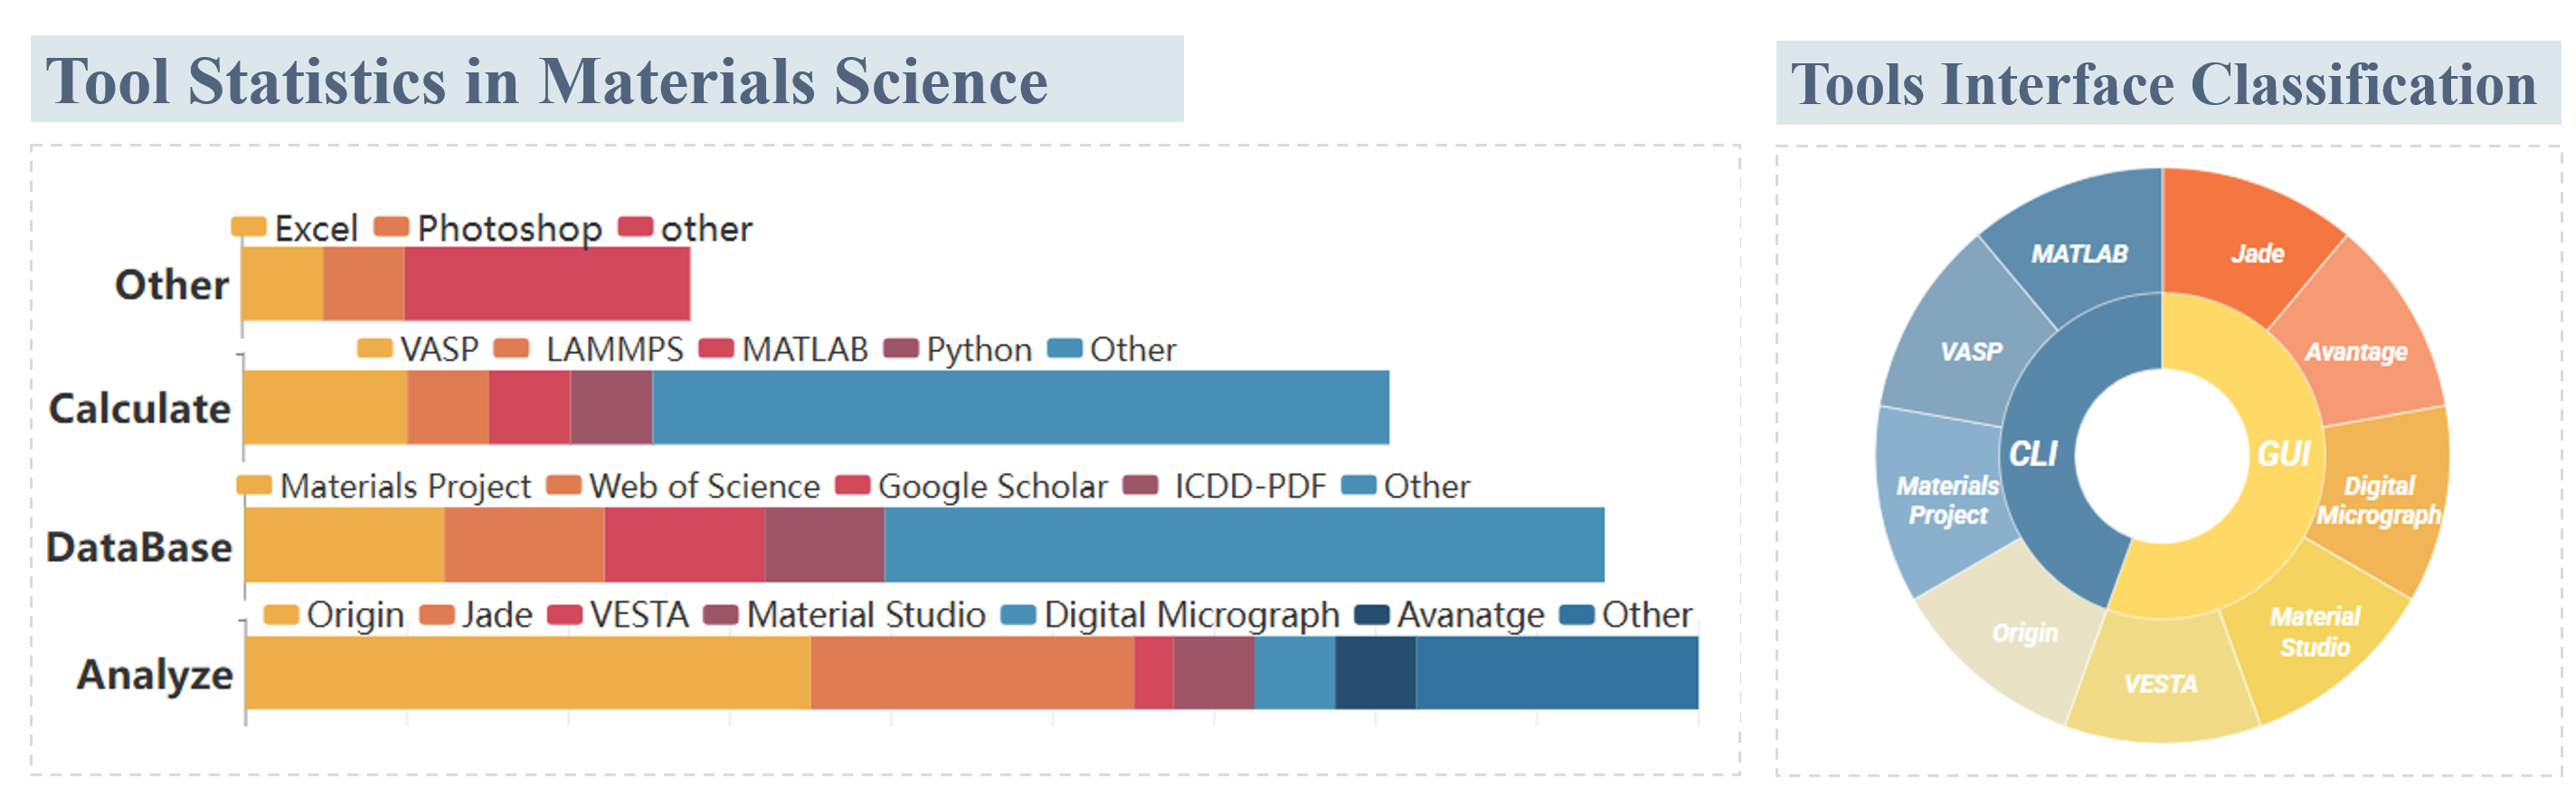
\includegraphics[width=\linewidth]{figures/introduction1.png}
    \caption{Survey results from 25 materials researchers:
    tool usage frequency across sub-fields (left) and
    distribution of primary interaction interface types (right).}
    \label{fig1}
  \end{minipage}
  \hfill
  \begin{minipage}[t]{0.48\linewidth}
    \centering
    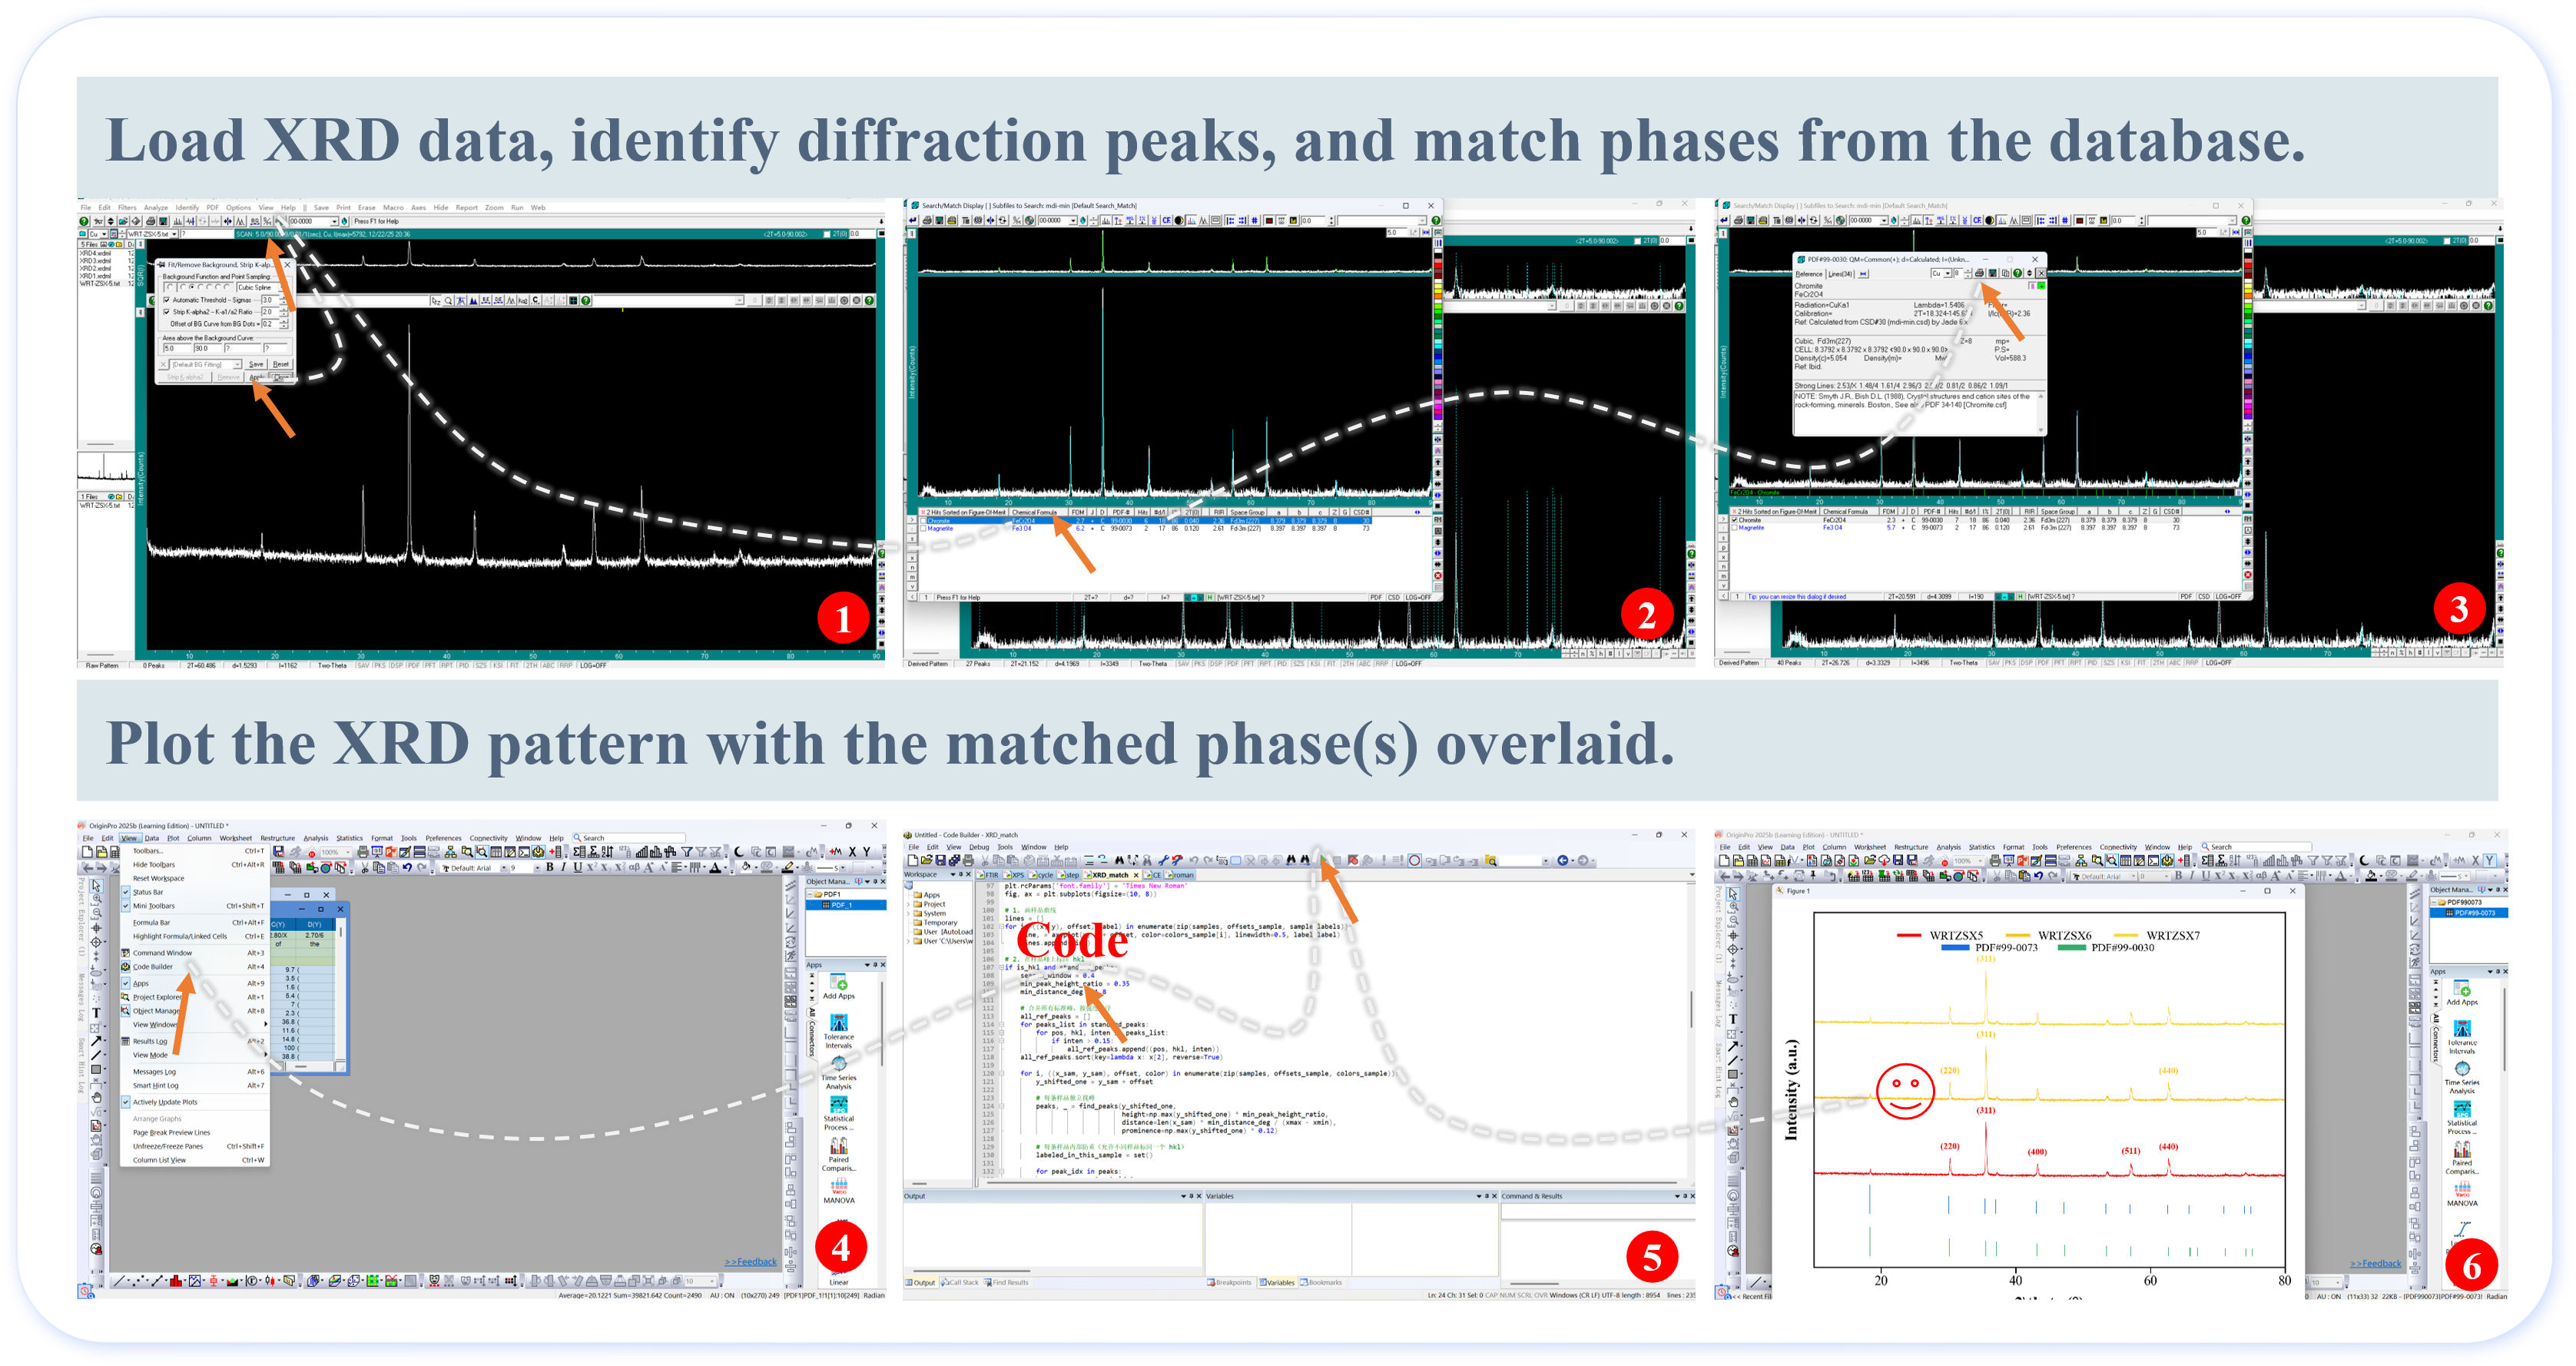
\includegraphics[width=\linewidth]{figures/introduction2.png}
    \caption{A complete XRD diffraction pattern requires cross-tool collaboration:
    raw XRD data is analyzed in JADE, then plotted and annotated in OriginPro.}
    \label{fig2}
  \end{minipage}
\end{figure*}

We present \textbf{MatToolBench}, a real-environment benchmark for evaluating multimodal
GUI agents on professional materials science software.
It covers 10 tools and 204 tasks across GUI, code, and cross-tool interaction modalities,
and pairs them with a multi-level evaluation framework—
text-based OCR matching, visual-text hybrid assessment, LLM aesthetic judgment, and code matching—
all grounded in fine-grained, expert-designed scoring sub-criteria.
GUI evaluators achieve an average F1 of 0.98 (JADE 0.991, MS 0.994, Avantage 0.980, VESTA 0.979;
see Appendix Table~\ref{tab:per_task_detail}), and the decomposed sub-criteria
provide dense RL reward signals for future training.
\section{Related Work}

\subsection{GUI-based Agents}
GUI agent research has progressed through a gradual evolution from web and mobile to general desktop operating systems. WebArena~\cite{webarena} and Mind2Web~\cite{mind2web} established benchmarks for web browsing tasks, while AITW~\cite{aitw} focused on mobile GUI interaction. On the desktop side, OSWorld~\cite{osworld} introduced a cross-platform general benchmark, and WindowsAgentArena~\cite{windowsagentarena} further enhanced desktop perception through the Windows Accessibility Tree. Although ProSoftArena~\cite{prosoftarena} extended evaluation to professional creative software such as Adobe and Figma, its task objectives remain within the scope of general operations, and such software benefits from abundant interaction data and tutorials on the internet. 

Existing benchmarks have not yet addressed the GUI ecosystem of professional scientific domains. Unlike general-purpose or creative software, professional software in fields like materials science presents a dual challenge. First, due to its highly vertical nature, relevant interaction data and operational demonstrations on the web are extremely scarce, resulting in natural ``knowledge blind spots'' for general agents that rely on large-scale pre-training. Second, the operational logic of these tools extends far beyond basic interface interaction, deeply coupling with complex, domain-specific scientific knowledge. Consequently, existing benchmarks fail to measure the true performance of agents in data-scarce, knowledge-intensive real-world scientific workflows.

\subsection{Science Benchmarks}
Agent evaluation in the scientific domain has undergone a paradigm shift from knowledge reasoning to program execution. SciBench~\cite{scibench} and MatSciBench~\cite{matscibench} primarily rely on textual reasoning; ScienceAgentBench~\cite{scienceagentbench}, SciCode~\cite{scicode}, and MatTools~\cite{mattools} further incorporate code execution; while Spider2-V~\cite{spider2v}, ScienceBoard~\cite{scienceboard}, and LabBench~\cite{labbench} extend evaluation to multi-step workflows spanning multiple tools. However, all the aforementioned benchmarks evaluate agents exclusively through structured APIs, program code, or backend logs, without requiring genuine graphical interface perception or interaction capabilities. 

Although works such as CLI-Anything attempt to invoke software functionalities via command-line interfaces (CLIs), the professional tools widely used in scientific research (e.g., VESTA, Materials Studio, or Jade) inherently rely on complex 3D rendering, high-density information charts, and implicit visual feedback. These interactive dimensions fundamentally cannot be encapsulated or replaced by pure text or CLI interfaces. To bridge this critical gap, this work presents the first comprehensive multimodal agent benchmark for materials science, requiring models not only to possess scientific reasoning capabilities but also to execute professional software operations and cross-tool collaboration within realistic GUI environments.

\section{MatToolBench Environment}

As illustrated in Figure~\ref{fig3}, the \textsc{MatToolBench} environment is built on a
Windows~11 virtual machine and exposes three interaction modalities—GUI
operation, Python code generation, and OriginPro script authoring—through
a unified Gymnasium interface.

%%%%%%%%%%该图要重画，此处占位置
\begin{figure}
    \centering
    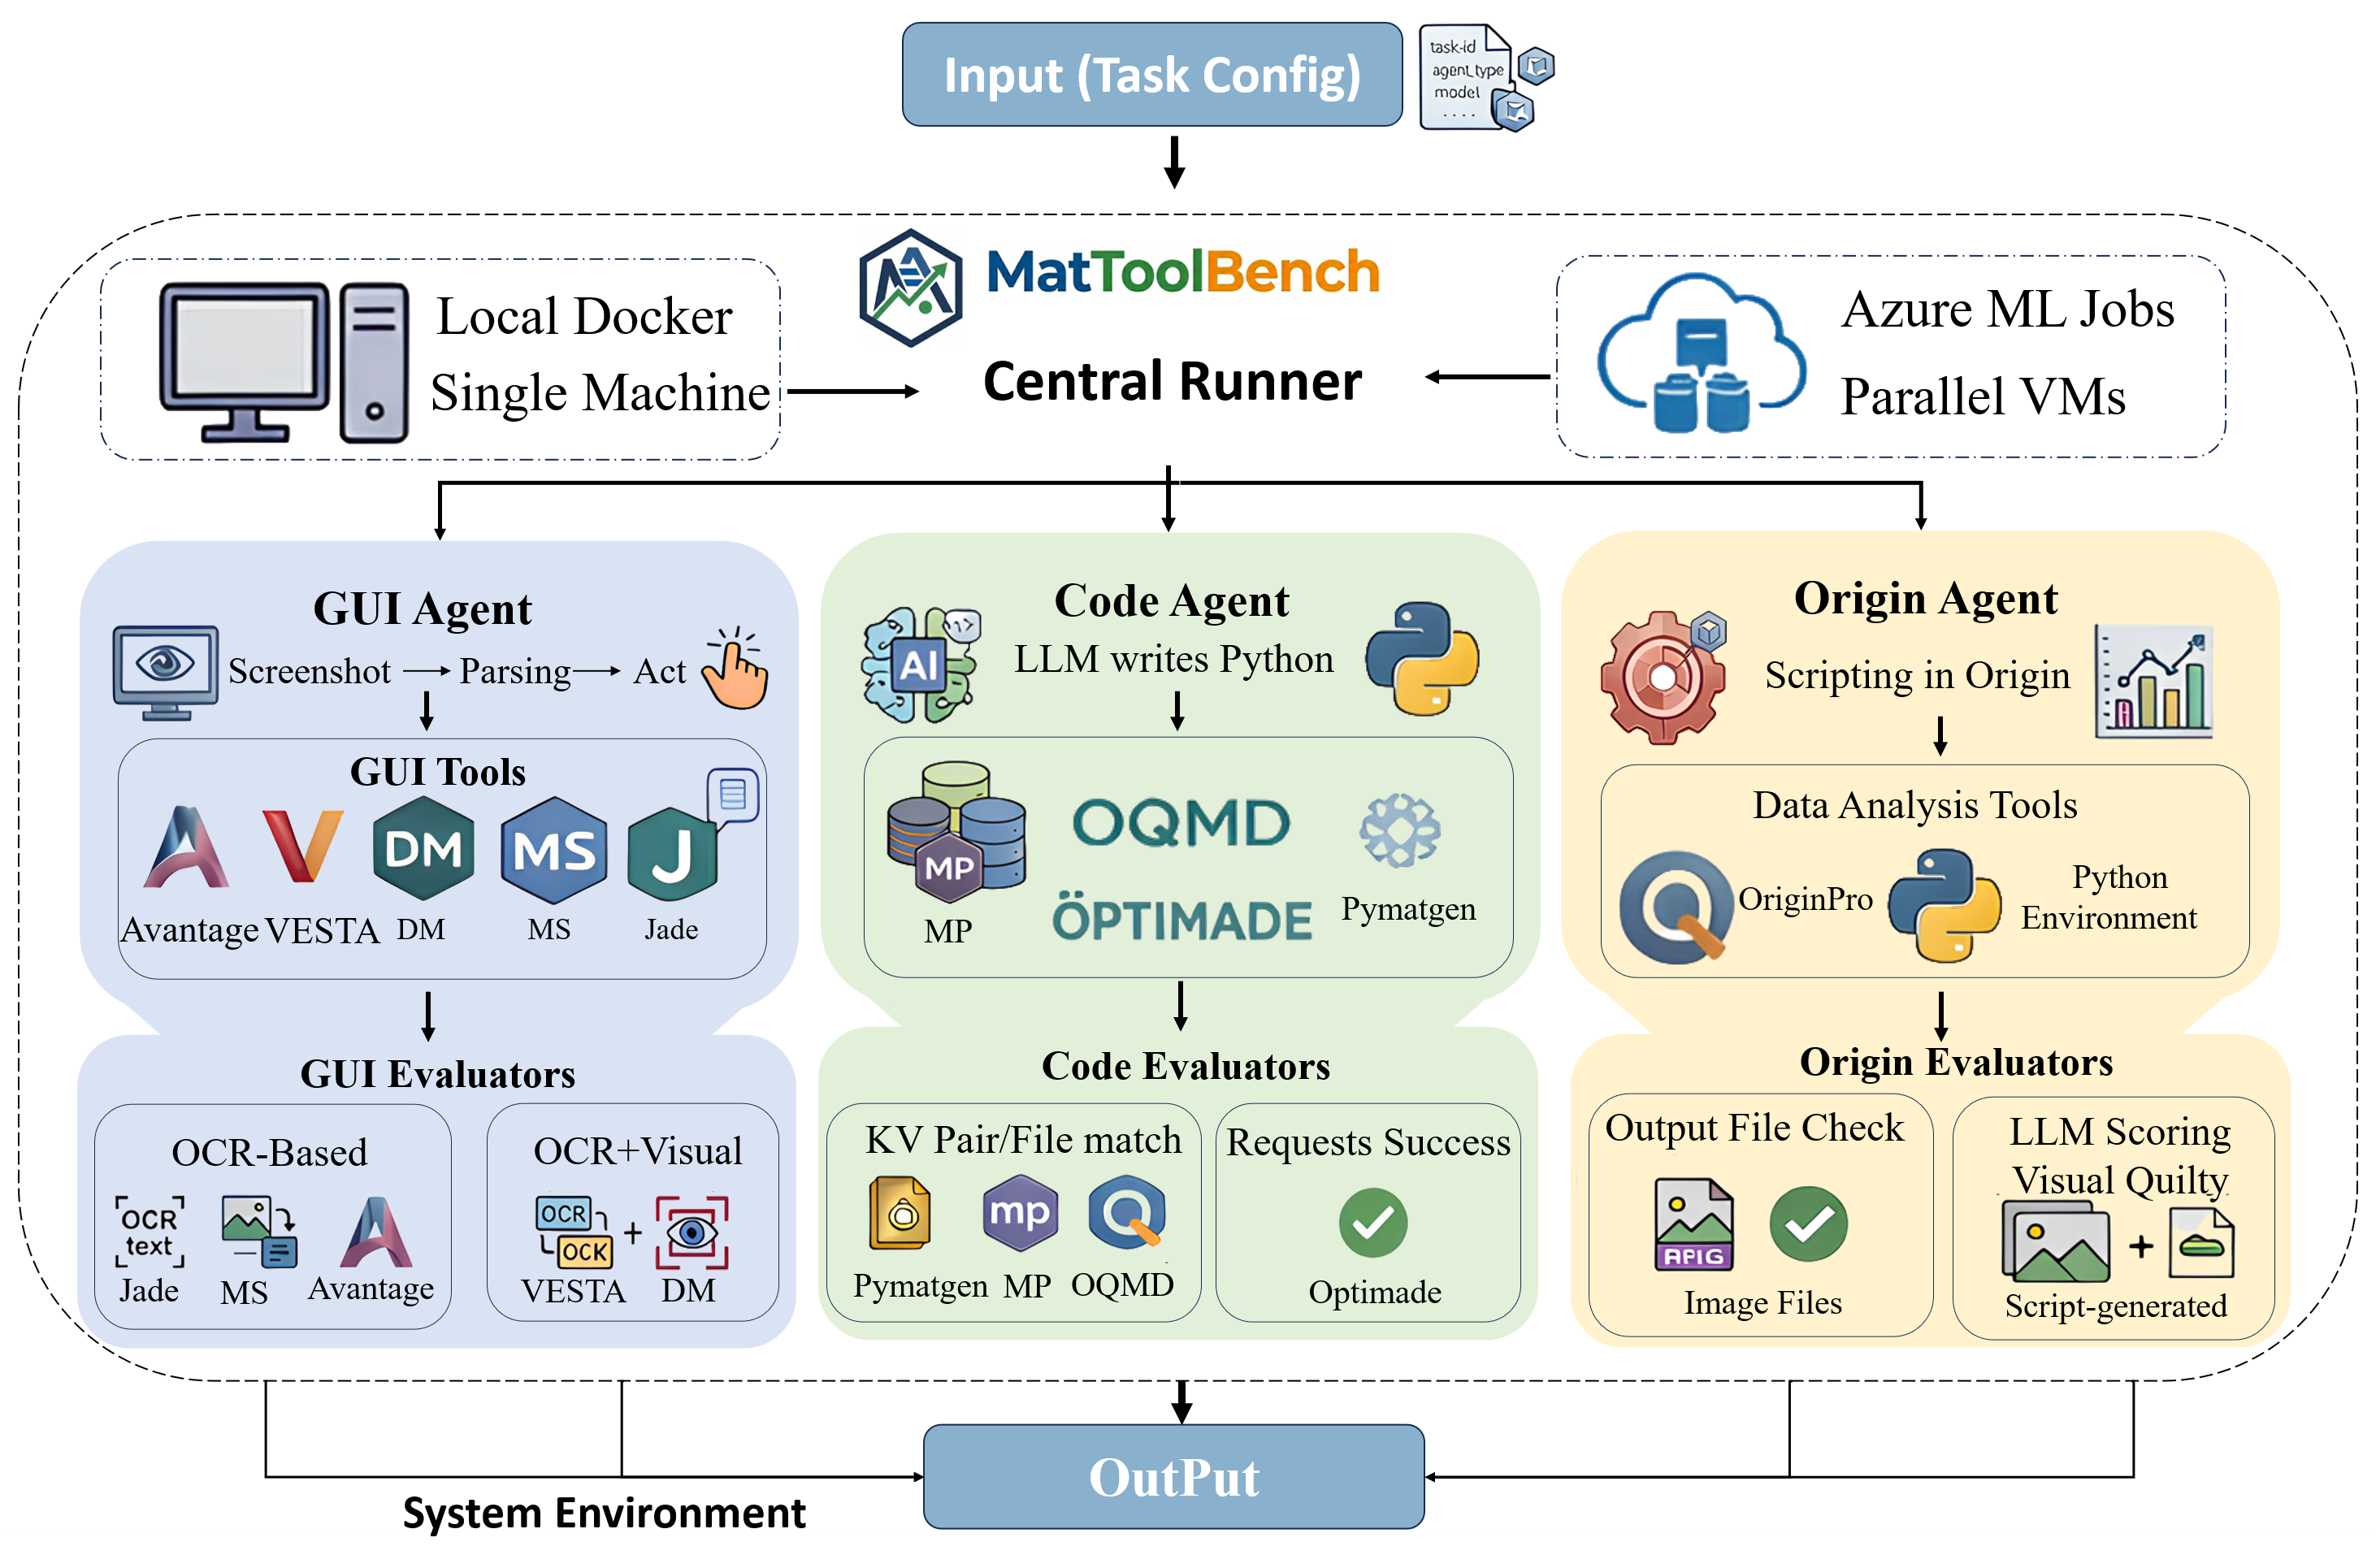
\includegraphics[width=1\linewidth]{figures/model.png}
    \caption{Overview of the \textsc{MatToolBench} framework.
    Tasks are dispatched by a central runner to one of three specialized agents:
    the \emph{GUI Agent} operates materials science desktop applications
    (e.g., JADE, VESTA, Avantage) via screenshot parsing and element grounding;
    the \emph{Code Agent} generates Python scripts to query materials database
    APIs (e.g., MP, OQMD, OPTIMADE);
    and the \emph{Origin Agent} combines GUI interaction with OriginPro script
    generation for experimental data plotting.
    All agents execute inside a Windows~11 VM hosted within a Docker container,
    communicating through a Flask-based control server.
    Task-specific evaluators assess the final environment state after each episode.}
    \label{fig3}
\end{figure}
%%%%%%%%%%该图要重画，此处占位置

\subsection{Task Definition}
Task execution is formalized as a POMDP
$\langle \mathcal{S}, \mathcal{O}, \mathcal{A}, \mathcal{T}, \mathcal{R} \rangle$.
At each step $t$ the agent receives observation $o_t$ (screenshot/execution feedback),
takes action $a_t$, and transitions to $s_{t+1}$.
Policy $\pi$ conditions on the full history
$m_t = \{g, o_0, a_0, \ldots, o_t\}$ where $g$ is the fixed natural-language instruction.
Episodes terminate on: \texttt{DONE} (agent declares success),
\texttt{FAIL} (agent declares infeasible), or step-budget exhaustion (default 50 for GUI/Origin,
10 for code). A \texttt{WAIT} action is available for slow GUI responses.

\paragraph{Reward Design for RL.}
A central design goal of \textsc{MatToolBench} is to serve as an
\emph{RL-friendly} training environment.
Rather than providing only a binary success/failure signal,
each task is decomposed into multiple \textbf{scoring sub-criteria}
(detailed in Section~4.1), each corresponding to a verifiable
intermediate or final state the agent must achieve.
Upon episode termination, the task-specific evaluator independently
assesses every sub-criterion and produces a fine-grained score vector,
from which the overall task score is computed as the fraction of
sub-criteria satisfied.
This decomposed reward structure yields substantially denser feedback
than a single binary outcome:
it tells the agent \emph{which} sub-goals were achieved and which were
missed, enabling more informative credit assignment during
policy optimization.
For tasks annotated as infeasible, the agent receives a score of $1$
only if it correctly emits \texttt{FAIL}.

\subsection{Observation Space}

\paragraph{GUI-Based Tasks.}
Each observation $o_t$ for desktop-application tasks is a configurable tuple comprising:
the task instruction $g$; a full-desktop screenshot $v_t$ (1920$\times$1080);
an optional UIA accessibility tree $e_t$; an optional Set-of-Marks (SoM) image $r_t$
in which UI regions from $e_t$, OmniParser~\cite{lu2024omniparser}, or both are
overlaid as numbered bounding boxes; foreground window metadata; and clipboard content.
Six \texttt{observation\_type} modes are supported, ranging from raw screenshot only
(\texttt{no\_omni}) to accessibility\,+\,OmniParser hybrid (\texttt{mixed-omni}).

\paragraph{Code and Origin Tasks.}
For database tasks (MP, OQMD, OPTIMADE, Pymatgen), $o_t$ reduces to text-only execution
feedback (\texttt{stdout}, \texttt{stderr}, return code); no visual signal is provided.
For Origin tasks, observations additionally include the current OriginPro workspace
screenshot, enabling the agent to verify whether the generated plot meets requirements.

\subsection{Action Space}

\paragraph{GUI Actions.}
GUI tasks use a hierarchical \texttt{Computer} interface with five sub-modules:
\texttt{Mouse} (element-ID or normalized-coordinate positioning, click, scroll, drag),
\texttt{Keyboard} (character input and hotkeys),
\texttt{Clipboard} (text/image copy-paste),
\texttt{OS} (program launch), and
\texttt{WindowManager} (fuzzy-match application switching).
Actions are transmitted as Python code strings executed via \texttt{exec()} on the VM;
the element-ID-based \texttt{move\_id()} reduces sensitivity to localization errors.
The full API is in Appendix Table~\ref{tab:computer_api}.

\paragraph{Code and Origin Actions.}
Code tasks reduce to a generate-and-correct loop: the agent writes a complete Python
script per step, executed in an isolated virtual environment per domain;
\texttt{stdout}/\texttt{stderr}/return-code are fed back for self-correction.
Origin tasks inject scripts into OriginPro's Code Builder via clipboard paste and \texttt{F5},
combining code generation with GUI navigation.

\subsection{Execution Environment}
The environment has two layers: an \textbf{outer} Linux Docker container for agent logic and
visual parsing (OmniParser), and an \textbf{inner} Windows~11 VM on QEMU/KVM
(1920$\times$1080) pre-installed with all target applications and isolated Python venvs per
code domain. A Flask HTTP server in the VM (port~5000) is the sole control interface;
external API calls route through a tinyproxy instance in the container.
Each episode resets by closing applications and running task-specific JSON setup scripts
(file download, app launch, window activation).
The framework exposes a standard Gymnasium interface (\texttt{reset()}, \texttt{step()},
\texttt{evaluate()}) and supports concurrent multi-worker evaluation.


\section{The \textsc{MatToolBench} Benchmark}

\subsection{Task Statistics}

\textsc{MatToolBench} comprises \textbf{204 tasks} spanning \textbf{10 domain-specific
tools}, organized into three agent types: GUI-based (JADE, Avantage, VESTA, DM, MS),
Origin-based (Origin), and code-based (MP, OQMD, OPTIMADE, Pymatgen, VASP).
Figure~\ref{fig:task-pie} illustrates the sub-category distribution within each domain.

\paragraph{Scoring Scheme.}
Each task is decomposed into one or more \textbf{scoring sub-criteria} (pts),
each corresponding to a distinct intermediate or final state the agent must
correctly achieve. The per-task score equals the fraction of sub-criteria satisfied,
enabling partial credit on multi-step tasks. A task is counted as a full success
(SR\,=\,1) only when all sub-criteria are met.

\paragraph{Difficulty Levels.}
Tasks are stratified into three levels based on the number of scoring sub-criteria,
which serves as a proxy for operational complexity:
\textbf{Easy} (1--3\,pts) involves single-step or few-step operations such as
file loading or single-function execution;
\textbf{Medium} (4\,pts) requires chained multi-step workflows with intermediate
verification; and
\textbf{Hard} (5--7\,pts) demands complex workflows combining multiple functions,
parameter configuration, and end-to-end result validation.

\begin{figure*}[t]
\centering
\begin{minipage}[c]{0.50\textwidth}
  \centering
  \footnotesize
  \renewcommand{\arraystretch}{1.35}
  \setlength{\tabcolsep}{4pt}
  \captionof{table}{Benchmark task statistics.
  E/M/H: easy\,/\,medium\,/\,hard (1--3\,/\,4\,/\,5--7\,pts).}
  \label{tab:task-stats}
  \begin{tabular}{lp{2.2cm}cccr}
  \toprule
  \textbf{Cat.} & \textbf{Domain} & \textbf{\#} & \textbf{E/M/H}
    & \textbf{Avg} & \textbf{Tot.} \\
  \midrule
  \multirow{5}{*}{GUI}
    & Avantage & 20 & 13/2/5            & 3.75 & 75 \\
    & DM       & 20 & 13/4/3            & 3.35 & 67 \\
    & JADE     & 20 & 14/3/3            & 3.45 & 69 \\
    & MS       & 20 & \phantom{0}6/6/8  & 4.10 & 82 \\
    & VESTA    & 20 & 13/2/5            & 3.45 & 69 \\
  \midrule
  Origin & Origin & 16 & ---             & 2.00 & 32 \\
  \midrule
  Code   & MP / OQMD / OPTIMADE / Pymatgen
                   & 80 & ---            & 1.00 & 80 \\
  \midrule
  Mixed  & Mixed   &  8 & ---            & ---  & --- \\
  \midrule
  \textbf{Total} & & \textbf{204} & & & \textbf{394+} \\
  \bottomrule
  \end{tabular}
\end{minipage}
\hfill
\begin{minipage}[c]{0.46\textwidth}
  \centering
  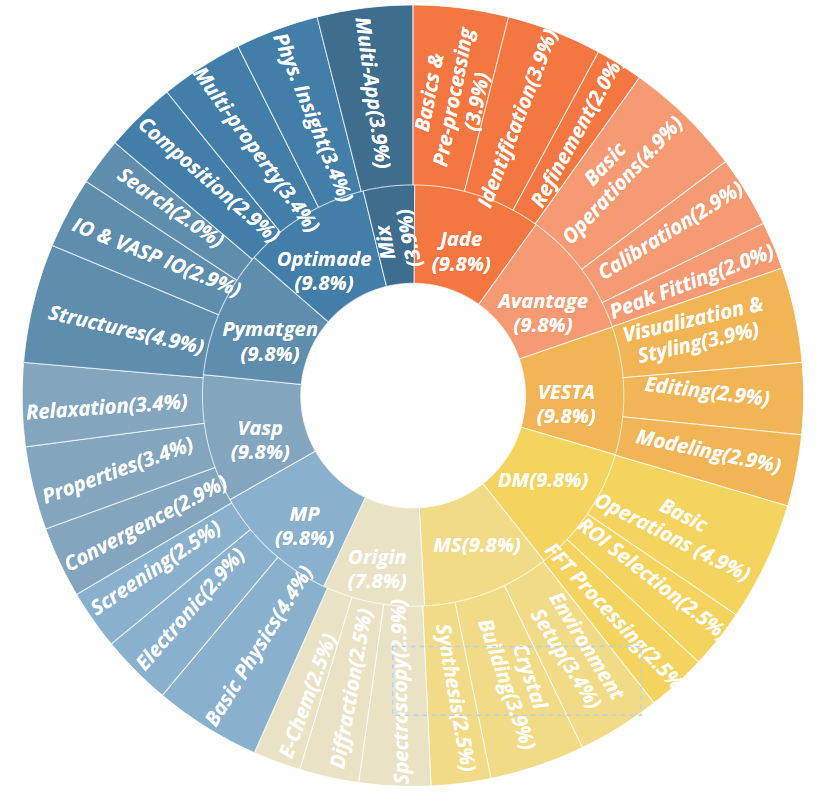
\includegraphics[width=\textwidth]{figures/pie.png}
  \captionof{figure}{Task distribution across all 10 domains and sub-categories.
  The inner ring shows domains; the outer ring shows sub-categories with their
  percentage of total tasks.}
  \label{fig:task-pie}
\end{minipage}
\end{figure*}

%% ────────────────────────────────────────────────────────────────────────────
\subsection{Evaluation Protocol}

Evaluation follows a two-stage pipeline after each episode: a domain-specific
\textbf{getter} extracts the task-relevant result, and a \textbf{metric function}
scores it against a reference. GUI results are extracted via OCR or pixel analysis;
code results are written to files and compared against a gold-standard directory;
Origin results use file-existence check plus an optional GPT-4o visual judge.
Metric details are in Appendix Tables~\ref{tab:eval-metrics}--\ref{tab:eval-gui-getters}.

\paragraph{Metrics.}
We report \textbf{Score} (normalized fraction of sub-criteria satisfied, enabling
partial credit) and \textbf{SR} (success rate: all sub-criteria met).
Efficiency is captured by \textbf{Eff*} (valid-action ratio on successful episodes)
and \textbf{FTR} (false termination rate: fraction of agent-terminated episodes where
SR\,=\,0), both computed over agent-terminated episodes only.



%% ────────────────────────────────────────────────────────────────────────────
\section{Experiments}
\label{sec:experiments}

\subsection{Experimental Setup}
\label{sec:setup}

\paragraph{Models.}
We evaluate seven state-of-the-art multimodal models spanning three commercial providers:
\textbf{doubao-seed-1-8} (ByteDance), \textbf{kimi-k2.5} (Moonshot), \textbf{Claude-sonnet-4.6} (Anthropic),
\textbf{GPT-5.4} (OpenAI), \textbf{qwen3-vl-235b} and \textbf{qwen-vl-32b} (Alibaba),
and \textbf{qwen3-vl-8b} (Alibaba).
All models are accessed via their respective official APIs.
For GUI and Origin tasks, each model is wrapped in the \textsc{NaviAgent} framework
with SoM-annotated screenshots (mixed-oss mode) and a system prompt tailored to the agent type;
for code tasks, no visual input is provided.
The maximum step budget is 50 for GUI/Origin tasks and 10 for code tasks.

\paragraph{Claude Coordinate Calibration.}
\label{sec:claude-coord}
During evaluation, we identified an important model-specific behavior in Claude-sonnet-4.6:
although screenshots are captured and transmitted at the native 1920$\times$1080 resolution,
Claude internally resizes images to 1456$\times$816 pixels before processing.
Without explicit correction, the model computes normalized click coordinates by dividing pixel
positions by 1920 and 1080, yielding systematically mis-calibrated coordinates
(a deviation of $\approx$24\% horizontally and $\approx$24\% vertically).
This causes nearly all element-level interactions to miss their targets, resulting in a dramatic
drop in task performance.
To address this, we inject the following calibration notice at the start of every Claude system prompt:

\begin{quote}\small\ttfamily
[CLAUDE\_COORD\_RULE\_ACTIVATED: 1456x816] \\
Claude internally resizes images to 1456\,$\times$\,816\,px. \\
Use \texttt{normalized\_x = pixel\_x / 1456}, \texttt{normalized\_y = pixel\_y / 816}. \\
Do NOT divide by 1920 or 1080.
\end{quote}

Without this correction, Claude-sonnet-4.6 achieves near-zero GUI success rates across all domains.
With it, the model recovers to competitive performance, as reported in Table~\ref{tab:results-accuracy}.
We emphasize that this is an inherent property of the Claude model family's vision pipeline
and is not specific to our benchmark; any GUI benchmark that requires precise coordinate-level
interactions should apply the same correction when evaluating Claude models.

\subsection{Main Results}
\label{sec:main-results}

%% ── 主实验准确性表 ───────────────────────────────────────────────────────────
\begin{table*}[t]
\centering
\small
\renewcommand{\arraystretch}{1.18}
\setlength{\tabcolsep}{4.5pt}
\caption{Accuracy results on \textsc{MatToolBench}.
Sc.~(Score): normalized task score (\%) averaged over sub-criteria;
SR: success rate (\%, all sub-criteria satisfied).
\textbf{Bold}: best per metric; \underline{underline}: second best.
Abbrev.: doubao\,seed-1.8\,=\,doubao-seed-1-8; Claude\,son.-4.6\,=\,Claude-sonnet-4.6;
Qwen3\,235B/8B\,=\,qwen3-vl-235b/8b; Qwen\,32B\,=\,qwen-vl-32b.}
\label{tab:results-accuracy}
\resizebox{\textwidth}{!}{%
\begin{tabular}{ll cc cc cc cc cc cc cc}
\toprule
& & \multicolumn{2}{c}{\makecell{\textbf{doubao}\\[-1pt]\textbf{seed-1.8}}}
    & \multicolumn{2}{c}{\makecell{\textbf{kimi}\\[-1pt]\textbf{k2.5}}}
    & \multicolumn{2}{c}{\makecell{\textbf{Claude}\\[-1pt]\textbf{son.-4.6}}}
    & \multicolumn{2}{c}{\makecell{\textbf{GPT}\\[-1pt]\textbf{-5.4}}}
    & \multicolumn{2}{c}{\makecell{\textbf{Qwen3}\\[-1pt]\textbf{235B}}}
    & \multicolumn{2}{c}{\makecell{\textbf{Qwen}\\[-1pt]\textbf{32B}}}
    & \multicolumn{2}{c}{\makecell{\textbf{Qwen3}\\[-1pt]\textbf{8B}}} \\
\cmidrule(lr){3-4}   \cmidrule(lr){5-6}   \cmidrule(lr){7-8}
\cmidrule(lr){9-10} \cmidrule(lr){11-12} \cmidrule(lr){13-14} \cmidrule(lr){15-16}
\textbf{Cat.} & \textbf{Domain}
  & \textbf{Sc.} & \textbf{SR}
  & \textbf{Sc.} & \textbf{SR}
  & \textbf{Sc.} & \textbf{SR}
  & \textbf{Sc.} & \textbf{SR}
  & \textbf{Sc.} & \textbf{SR}
  & \textbf{Sc.} & \textbf{SR}
  & \textbf{Sc.} & \textbf{SR} \\
\midrule
\multirow{6}{*}{GUI}
  & Avantage & \textbf{44.6} & \textbf{35.0} & 32.3 & \underline{20.0} & \underline{41.3} & \textbf{35.0} & 32.3 & 15.0 & 30.8 & 10.0 & 26.2 & 15.0 & 18.5 & 15.0 \\
  & JADE     & \underline{54.2} & \textbf{25.0} & 50.8 & \textbf{25.0} & \textbf{57.6} & \textbf{25.0} & 50.8 & \underline{20.0} & 45.8 & 10.0 & 37.3 & 10.0 & 37.3 & 5.0 \\
  & DM       & \textbf{56.7} & \textbf{20.0} & \underline{52.2} & \textbf{20.0} & 40.3 & \textbf{20.0} & 50.7 & \textbf{20.0} & \underline{52.2} & \underline{10.0} & 6.0 & 0.0 & 38.8 & \underline{10.0} \\
  & MS       & 47.6 & 15.0 & 35.4 & 10.0 & \underline{52.4} & \underline{20.0} & \textbf{56.1} & \textbf{30.0} & 43.9 & 0.0 & 26.8 & 0.0 & 20.7 & 0.0 \\
  & VESTA    & 52.2 & \underline{20.0} & \underline{59.4} & \textbf{25.0} & 58.0 & \textbf{25.0} & \textbf{65.2} & \underline{20.0} & 52.2 & 10.0 & 29.0 & 10.0 & 30.4 & 10.0 \\
\cmidrule(lr){2-16}
\rowcolor[gray]{0.93}
  & \textit{Avg.} & \textbf{52.1} & \underline{24.0} & 46.0 & 20.0 & 49.9 & \textbf{25.0} & \underline{51.0} & 21.0 & 45.0 & 8.0 & 25.1 & 7.0 & 29.1 & 8.0 \\
\midrule
\rowcolor[gray]{0.93}
Origin & (pending) & --- & --- & --- & --- & --- & --- & --- & --- & --- & --- & --- & --- & --- & --- \\
\midrule
\multirow{5}{*}{Code}
  & Pymatgen & 30.0 & 30.0 & 15.0 & 15.0 & 25.0 & 25.0 & \textbf{35.0} & \textbf{35.0} & \textbf{35.0} & \textbf{35.0} & \underline{29.4} & \underline{29.4} & 15.0 & 15.0 \\
  & MP       & \textbf{25.0} & \textbf{25.0} & \underline{22.5} & \underline{20.0} & 21.9 & 15.0 & 17.5 & 15.0 & \textbf{25.0} & \textbf{25.0} & 10.0 & 10.0 & 10.0 & 10.0 \\
  & OQMD     & 33.2 & 10.0 & 50.3 & 30.0 & \textbf{60.8} & \textbf{50.0} & \underline{58.2} & \underline{45.0} & 26.2 & 10.0 & 11.5 & 0.0 & 18.4 & 0.0 \\
  & OPTIMADE & 70.0 & 70.0 & \underline{80.0} & \underline{80.0} & 75.0 & 75.0 & \textbf{85.0} & \textbf{85.0} & 20.0 & 20.0 & 30.0 & 30.0 & 10.0 & 10.0 \\
\cmidrule(lr){2-16}
\rowcolor[gray]{0.93}
  & \textit{Avg.} & 39.6 & 33.8 & 42.0 & 36.2 & \underline{45.7} & \underline{41.3} & \textbf{48.9} & \textbf{45.0} & 26.6 & 22.5 & 20.2 & 17.4 & 13.4 & 8.8 \\
\midrule
\rowcolor[gray]{0.93}
\multicolumn{2}{l}{\textbf{Overall Avg.}}
  & --- & --- & --- & --- & --- & --- & --- & --- & --- & --- & --- & --- & --- & --- \\
\bottomrule
\end{tabular}%
}
\end{table*}

Table~\ref{tab:results-accuracy} reports Score and SR for all seven models across GUI, Origin,
and Code domains.
The overall performance level is consistently low, with the best-performing models
achieving only 24--25\% SR on GUI tasks and 41--45\% SR on code tasks,
highlighting the substantial difficulty of professional materials science workflows
relative to general GUI benchmarks.

\paragraph{GUI Tasks.}
The top performers on GUI tasks are doubao-seed-1-8 and GPT-5.4,
achieving average SRs of 24.0\% and 21.0\% respectively.
Claude-sonnet-4.6 ranks second overall with an average SR of 25.0\%,
benefiting from strong visual grounding once the coordinate calibration (Section~\ref{sec:claude-coord})
is applied.
Models without adequate GUI grounding — notably qwen-vl-32b (7.0\% avg.\ SR) —
struggle on tasks requiring precise multi-step interaction sequences.

Among individual domains, \textbf{MS} (Materials Studio) is consistently the most challenging,
with all models except GPT-5.4 scoring below 20\% SR.
This reflects Materials Studio's highly nested menu hierarchy and implicit feedback after operations.
In contrast, \textbf{VESTA} and \textbf{JADE} show relatively higher scores,
likely because these tools provide more explicit visual confirmation of state changes.

A notable gap exists between Score and SR across all GUI domains:
models routinely complete a fraction of scoring sub-criteria (e.g., Score\,$\approx$50\%)
while rarely satisfying all of them simultaneously (SR\,$\approx$20\%).
This pattern confirms the utility of the partial-credit scoring mechanism:
it reveals that models \emph{do} make meaningful progress on complex tasks,
even when they fall short of full completion.

\paragraph{Code Tasks.}
Code tasks show higher performance overall, consistent with LLMs' strength in structured
text generation.
GPT-5.4 achieves the best average SR of 45.0\%, followed by Claude-sonnet-4.6 (41.3\%).
Performance varies markedly across databases:
\textbf{OPTIMADE} (a standardized REST query interface) yields the highest SRs (20--85\%),
because its query syntax is consistent and well-documented in pretraining data.
\textbf{MP} is more challenging (10--25\% SR) as it requires accurate use of
the \texttt{mp-api} Python client with evolving API conventions.
\textbf{OQMD} tasks occupy a middle ground (0--50\% SR), with large performance gaps
between frontier models (Claude 50\%, GPT 45\%) and smaller ones (Qwen-8b 0\%).

The smaller Qwen models (32b, 8b) underperform substantially on code tasks
despite reasonable GUI scores, suggesting that scientific API usage demands
domain-specific knowledge that scales differently from general GUI interaction.

\paragraph{Efficiency.}
Appendix Table~\ref{tab:results-efficiency} reports Eff/Eff* and FTR.
GUI tasks show moderate efficiency ($\approx$20--30\% Eff) reflecting frequent
exploratory actions, while code tasks reach $\approx$96\% Eff* since each step is a
complete script execution.
High FTR values (40--70\%) on GUI tasks reveal a persistent premature-termination
failure mode across all models.

\subsection{Origin Task Evaluation}
\label{sec:origin-eval}

Origin tasks require the agent to generate a publication-quality scientific figure
from raw experimental data using OriginPro.
Each task is evaluated along two axes:
(1) \textbf{file existence} — verified via \texttt{exact\_match}, checking that the output
\texttt{.png} is saved to the specified path;
and (2) \textbf{visual conformance} — assessed by a GPT-4o judge, which receives the generated
figure and a natural-language description of the expected visual result
(e.g., ``galvanostatic long-cycle voltage-time curve with annotation `5 mA cm\textsuperscript{$-2$}'''
and returns a binary pass/fail judgment.
This two-stage design distinguishes between agents that successfully run scripts versus
those that additionally produce figures that are visually and scientifically correct.

To complement the binary pass/fail judgment,
Figure~\ref{fig:radar-origin-quality} presents a multi-dimensional quality assessment
of Origin-generated figures across four task types (Raman, XRD, XPS, FTIR).
Nine human evaluators and four frontier LLMs
(GPT-4.5, Gemini-2.5-pro, doubao-seed-1-8, qwen3-vl-235b)
independently scored each figure on a 1--5 scale across three dimensions:
\textbf{visual correctness} (axes, units, data representation),
\textbf{aesthetic quality} (line style, color, layout),
and \textbf{task completeness} (all required elements present).
Our template-guided Origin agent achieves the highest scores across all dimensions,
validating both the quality of the reference template scripts and the effectiveness
of the evaluation framework.
Human and LLM evaluators show high agreement (Pearson $r > 0.91$),
confirming that the LLM-based aesthetic judge is a reliable proxy for human judgment.

\subsection{Ablation Study: Effect of Prompt Templates}
\label{sec:ablation}

We ablate the effect of domain-specific prompt hints (\texttt{hint\_mode})
by comparing the full agent prompt against a \texttt{no\_hint} baseline
that omits all domain-specific workflow instructions,
evaluated on doubao-seed-1-8 and GPT-5.4.

Figure~\ref{fig:ablation} summarizes the results.
\textbf{Removing hints consistently degrades performance on GUI tasks}:
doubao-seed-1-8 drops from 35.0\% to 20.0\% SR on Avantage, from 25.0\% to 5.0\% on JADE,
and from 20.0\% to 0.0\% on DM.
This confirms that professional software workflows benefit substantially from
step-by-step operational guidance injected into the prompt.

On \textbf{code tasks}, the picture is more nuanced.
For OPTIMADE, both models retain nearly the same SR with and without hints
(doubao-seed-1-8: 70\% $\to$ 70\%; GPT-5.4: 85\% $\to$ 75\%),
suggesting that the structured query syntax of this database is sufficiently
learned by frontier models.
However, on MP and OQMD, removing hints causes larger drops
(GPT-5.4 MP: 15\% $\to$ 0\%), indicating that database-specific API conventions
are less well-covered in pretraining data and benefit from explicit hint injection.

The asymmetric effect of hints across task types reflects a key property of
domain-specific benchmarks: general-purpose models have uneven coverage of
specialized tool ecosystems, and targeted prompt engineering can partially
compensate for this knowledge gap.

\begin{figure}[tb]
  \centering
  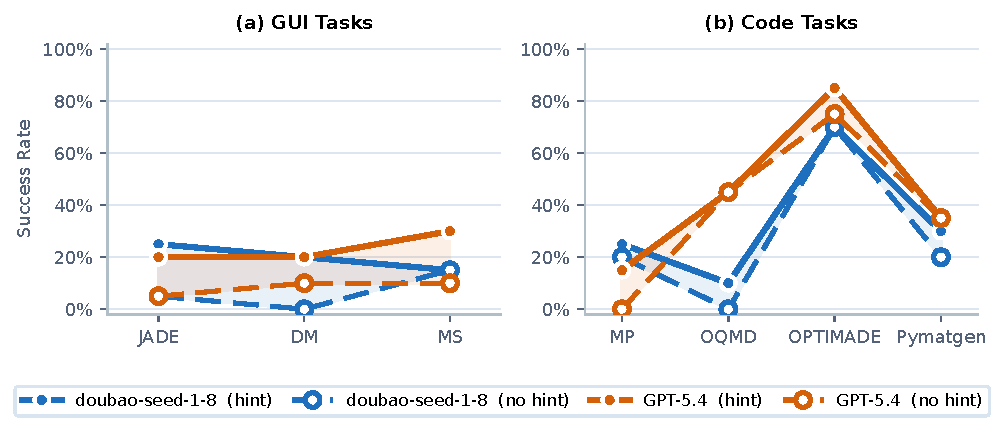
\includegraphics[width=\linewidth]{figures/ablation.pdf}
  \caption{Ablation study: SR comparison between \textbf{hint} (solid) and
  \textbf{no\_hint} (dashed) prompt modes for doubao-seed-1-8 (blue) and GPT-5.4 (orange).
  Left: GUI tasks. Right: Code tasks.
  Shaded bands indicate the gap between hint and no\_hint conditions.}
  \label{fig:ablation}
\end{figure}

\begin{table}[t]
\centering
\caption{Evaluator reliability for four GUI domains: aggregated Acc./Prec./Rec./F1 of the
  ground-truth getter pipeline. ``Score'' metrics validate value extraction;
  ``Software'' metrics validate software-state identification.
  Per-task breakdown is in Appendix Table~\ref{tab:per_task_detail}.}
\label{tab:overall}
\small
\begin{tabular}{lcccccccc}
\toprule
& \multicolumn{4}{c}{\textbf{Score}} & \multicolumn{4}{c}{\textbf{Software}} \\
\cmidrule(lr){2-5} \cmidrule(lr){6-9}
\textbf{Domain} & Acc. & Prec. & Rec. & F1 & Acc. & Prec. & Rec. & F1 \\
\midrule
JADE      & 1.00 & 1.00 & 0.99 & 0.99 & 1.00 & 1.00 & 1.00 & 1.00 \\
MS        & 1.00 & 0.99 & 1.00 & 0.99 & 1.00 & 1.00 & 1.00 & 1.00 \\
Avantage  & 0.99 & 0.98 & 0.98 & 0.98 & 1.00 & 0.98 & 1.00 & 0.99 \\
VESTA     & 0.98 & 0.94 & 0.99 & 0.97 & 0.99 & 0.94 & 1.00 & 0.97 \\
\bottomrule
\end{tabular}
\end{table}

\begin{figure}[t]
  \centering
  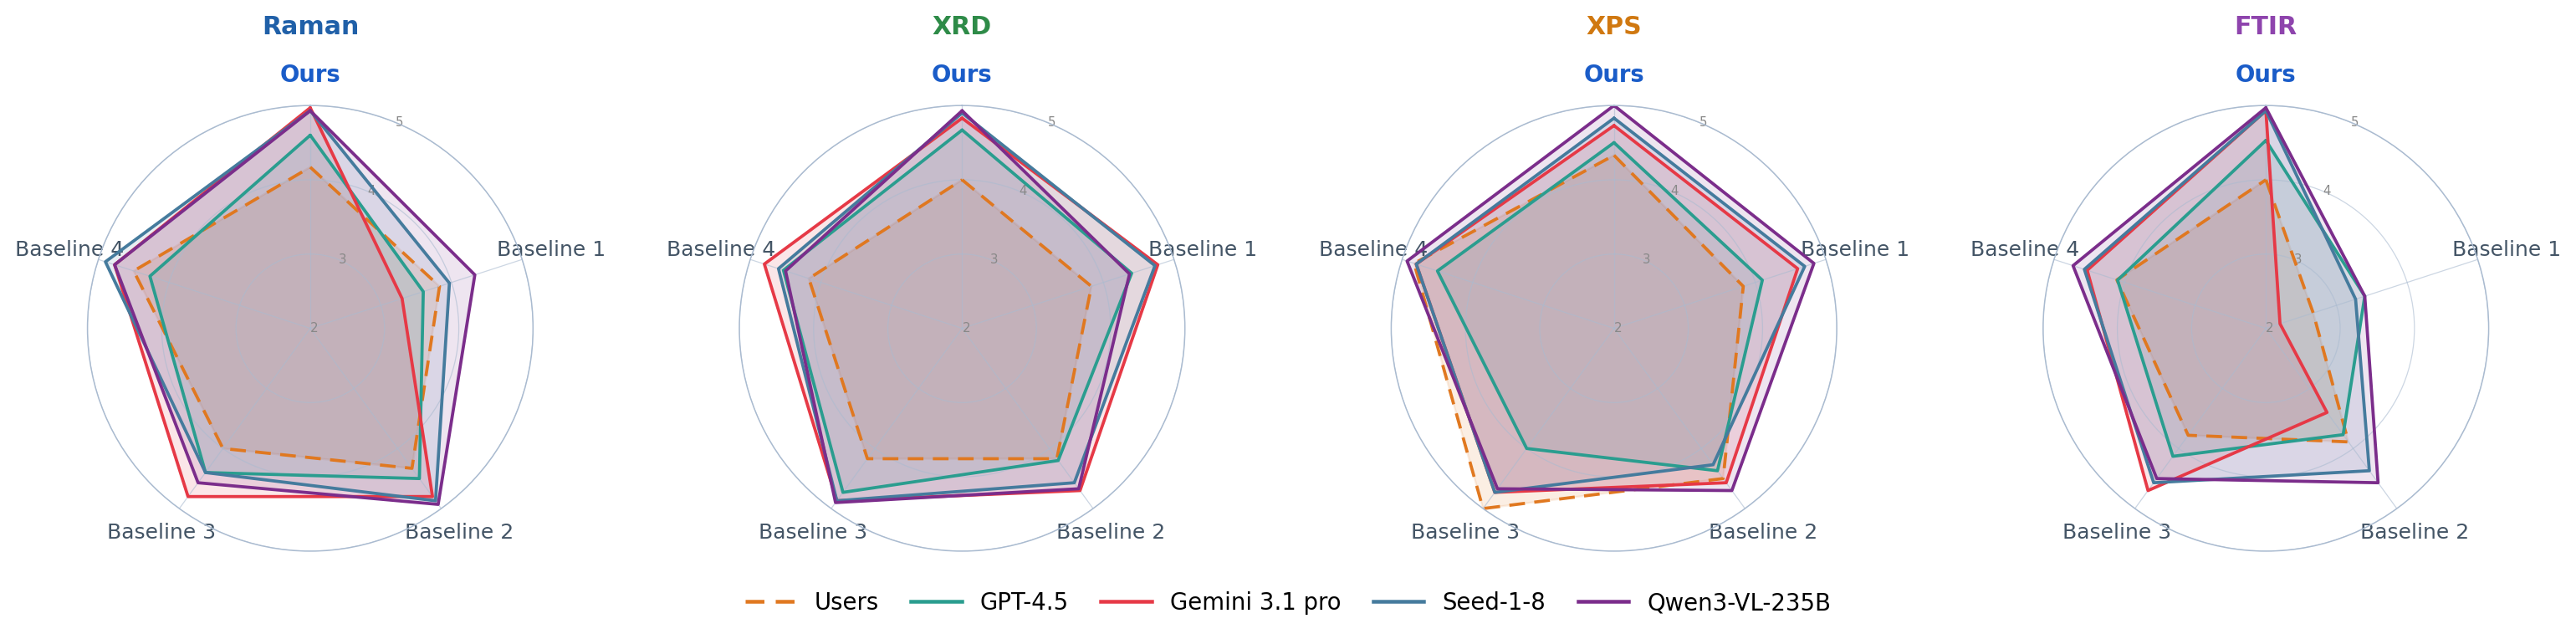
\includegraphics[width=\linewidth]{figures/radar_quality.png}
  \caption{Radar chart comparing Origin figure quality across four task types
    (Raman, XRD, XPS, FTIR). Each axis scores one method (1--5 scale) on three
    dimensions: visual correctness, aesthetic quality, and task completeness.
    Evaluations by 9 human raters (dashed) and four LLMs
    (GPT-4.5, Gemini-2.5-pro, Seed-1.8, Qwen3-235B);
    Pearson $r>0.91$ confirms LLM judges are reliable proxies for human judgment.}
  \label{fig:radar-origin-quality}
\end{figure}

\clearpage

\begin{ack}
Use unnumbered first level headings for the acknowledgments. All acknowledgments
go at the end of the paper before the list of references. Moreover, you are required to declare
funding (financial activities supporting the submitted work) and competing interests (related financial activities outside the submitted work).
More information about this disclosure can be found at: \url{https://neurips.cc/Conferences/2026/PaperInformation/FundingDisclosure}.


Do {\bf not} include this section in the anonymized submission, only in the final paper. You can use the \texttt{ack} environment provided in the style file to automatically hide this section in the anonymized submission.
\end{ack}

\bibliographystyle{plainnat}
\bibliography{ref}


%%%%%%%%%%%%%%%%%%%%%%%%%%%%%%%%%%%%%%%%%%%%%%%%%%%%%%%%%%%%

\appendix
\section{Action Space}

\begin{table}[h]
\centering
\caption{Complete action interface of the \texttt{Computer} object executed on the Windows VM.
  Each call is transmitted as a Python code string via HTTP POST and evaluated with
  \texttt{exec(code, \{"computer": computer\})} on the VM server.
  $^\dagger$\,\texttt{drag} accepts raw screen pixel coordinates, unlike \texttt{move\_abs}.
  $^\ddagger$\,\texttt{write} uses \texttt{pyautogui.write()} which is ASCII-only;
  use \texttt{clipboard.copy\_text()} for any multi-line or Unicode content.}
\label{tab:computer_api}
\small
\resizebox{\textwidth}{!}{%
\begin{tabular}{lllp{6cm}}
\toprule
\textbf{Module} & \textbf{Method} & \textbf{Parameters} & \textbf{Description} \\
\midrule
\multirow{7}{*}{\texttt{mouse}}
  & \texttt{move\_id(id)}      & Element ID (int)              & Move cursor to the bounding-box center of the SoM-annotated element with the given ID \\
  & \texttt{move\_abs(x, y)}   & Normalized coords $\in[0,1]$  & Move cursor to a relative screen position; $(0,0)$=top-left, $(1,1)$=bottom-right \\
  & \texttt{single\_click()}   & —                             & Left single-click at the current cursor position \\
  & \texttt{double\_click()}   & —                             & Left double-click at the current cursor position \\
  & \texttt{right\_click()}    & —                             & Right-click at the current cursor position \\
  & \texttt{scroll(dir)}       & \texttt{"up"} / \texttt{"down"} & Scroll the active window by 400 units in the given direction \\
  & \texttt{drag(x, y)}$^\dagger$ & Screen pixel coords (int)  & Left-button drag from current position to the target screen coordinates \\
\midrule
\multirow{2}{*}{\texttt{keyboard}}
  & \texttt{write(text)}$^\ddagger$ & ASCII string            & Type text character-by-character via \texttt{pyautogui.write()}; suitable only for short labels and filenames \\
  & \texttt{press(key)}        & Key name or combo           & Press a single key (e.g.\ \texttt{"f5"}, \texttt{"enter"}) or hotkey combo (e.g.\ \texttt{"ctrl+a"}, \texttt{"alt+4"}) \\
\midrule
\multirow{4}{*}{\texttt{clipboard}}
  & \texttt{copy\_text(text)}  & Unicode string (optional)   & Copy \textit{text} to the system clipboard via \texttt{pyperclip.copy()}; supports full Unicode. If called with no argument, sends \texttt{Ctrl+C} to copy the current selection \\
  & \texttt{paste()}           & —                           & Paste clipboard content at the current focus via \texttt{Ctrl+V} \\
  & \texttt{view\_clipboard()} & —                           & Return the current clipboard text as a Python string (via \texttt{pyperclip.paste()}) \\
  & \texttt{copy\_image(id)}   & Element ID (int)            & Crop the SoM element's bounding box from the screenshot and write it to the clipboard as a DIB bitmap via \texttt{win32clipboard} \\
\midrule
\multirow{3}{*}{\texttt{os}}
  & \texttt{open\_program(name)}    & Executable name (str) & Launch the named program via \texttt{start}, then maximize and bring to foreground; no-op if not installed \\
  & \texttt{maximize\_window()}     & Window handle (opt.)  & Maximize the specified window, or the current foreground window if omitted, via \texttt{win32gui} \\
  & \texttt{is\_installed(name)}    & Executable name (str) & Return \texttt{True} if the program is found in the Windows registry or PATH \\
\midrule
\multirow{2}{*}{\texttt{window\_manager}}
  & \texttt{switch\_to\_application(name)} & App name (str) & Restore and maximize the closest-matching visible window (fuzzy match via \texttt{difflib}), then bring it to the foreground \\
  & \texttt{find\_open\_applications()}    & —              & Return a list of title strings for all currently visible, non-empty windows \\
\bottomrule
\end{tabular}%
}
\end{table}

\section*{Appendix: Evaluation Protocol Details}

\begin{table}[ht]
\centering
\caption{Metric functions used per domain. \cmark: all tasks use this metric;
fractions indicate partial usage.}
\label{tab:eval-metrics}
\small
\begin{tabular}{lccc}
\toprule
\textbf{Domain} & \texttt{exact\_match} & \texttt{detect\_kv\_match} & \texttt{detect\_file\_match} \\
\midrule
Avantage  & \cmark & --     & --     \\
DM        & \cmark & --     & --     \\
JADE      & \cmark & --     & --     \\
MS        & \cmark & --     & --     \\
VESTA     & \cmark & --     & --     \\
Origin    & \cmark & --     & --     \\
MP        & --     & 14/20  & 6/20   \\
OQMD      & --     & \cmark & --     \\
OPTIMADE  & \cmark & --     & --     \\
Pymatgen  & --     & --     & \cmark \\
\bottomrule
\multicolumn{4}{p{0.85\columnwidth}}{%
\footnotesize
\textit{exact\_match}: binary $\{0,1\}$ outcome for discrete GUI results and
binary conditions. \quad
\textit{detect\_kv\_match}: parses key-value pairs and matches numeric values
within $r_\text{tol}=0.1\%$, returning partial credit. \quad
\textit{detect\_file\_match}: line-by-line comparison against a gold-standard
reference file, returning a binary outcome.}
\end{tabular}
\end{table}

\begin{table*}[ht]
\centering
\caption{Getter types used in GUI-based domains, all paired with \texttt{exact\_match}.}
\label{tab:eval-gui-getters}
\small
\resizebox{\textwidth}{!}{%
\begin{tabular}{llp{9cm}}
\toprule
\textbf{Domain} & \textbf{Getter Type} & \textbf{Description} \\
\midrule
\multirow{6}{*}{Avantage}
  & \texttt{check\_multiple\_files\_imported} & Confirms that multiple XPS scan channels (\textit{e.g.}, C\,1s, O\,1s, Zn\,2p) are loaded. \\
  & \texttt{check\_dialog\_exists}            & Detects the presence of a specific dialog window via OCR. \\
  & \texttt{check\_dialog\_parameter}         & Extracts and validates a parameter value inside a dialog. \\
  & \texttt{check\_stacked\_graph}            & Verifies that spectra are displayed in stacked mode. \\
  & \texttt{check\_background\_added}         & Confirms background curve addition to a spectrum. \\
  & \texttt{check\_energy\_axis\_reversed}    & Validates that the binding-energy axis is inverted. \\
\midrule
\multirow{6}{*}{DM}
  & \texttt{check\_file\_import}             & Verifies that a \texttt{.dm3}/\texttt{.dm4} file is imported. \\
  & \texttt{check\_ocr\_text}               & Extracts arbitrary text from the UI via OCR and matches it against an expected string. \\
  & \texttt{check\_drawing\_tool}           & Confirms the active drawing tool (box, circle, line, \textit{etc.}). \\
  & \texttt{check\_border\_color}           & Detects the border color of a drawn shape via pixel analysis. \\
  & \texttt{check\_roi\_copy\_and\_enlarge} & Verifies ROI duplication and enlargement. \\
  & \texttt{check\_checkbox\_selected}      & Confirms a checkbox state from the accessibility tree. \\
\midrule
\multirow{8}{*}{JADE}
  & \texttt{check\_file\_opened\_jade}   & Confirms that the target XRD data file is open. \\
  & \texttt{check\_peak\_finding}        & Counts the number of detected peaks in the XRD pattern. \\
  & \texttt{check\_background\_removal}  & Validates background subtraction by detecting a $\geq$20\% drop in $I_{\max}$. \\
  & \texttt{check\_smoothing}            & Confirms the ``Smooth whole Pattern'' operation. \\
  & \texttt{check\_axis\_switch}         & Verifies switching between two-theta and $d$-scale axes. \\
  & \texttt{check\_wpf\_refinement}      & Extracts the $R$-factor from Whole Pattern Fitting. \\
  & \texttt{check\_refinement\_result}   & Counts Rietveld refinement profiles. \\
  & \texttt{check\_dialog\_title\_jade}  & Matches expected dialog titles via OCR. \\
\midrule
\multirow{5}{*}{MS}
  & \texttt{check\_file\_in\_title}    & Confirms the project filename in the window title bar. \\
  & \texttt{check\_text\_keyword}      & Searches for specific keywords in UI panels (\textit{e.g.}, ``3D Atomistic''). \\
  & \texttt{check\_dialog\_title\_ms}  & Matches dialog titles with optional forbidden-keyword filters. \\
  & \texttt{check\_field\_value}       & Extracts and validates form-field values (\textit{e.g.}, space group ``P1''). \\
  & \texttt{check\_visual\_similarity} & Computes SSIM between the current screenshot and a reference image. \\
\midrule
\multirow{8}{*}{VESTA}
  & \texttt{check\_file\_opened\_vesta}   & Verifies that a CIF structure file is loaded. \\
  & \texttt{check\_dialog\_opened\_vesta} & Confirms a dialog window is visible. \\
  & \texttt{check\_atom\_deletion}        & Validates that specified atoms have been removed. \\
  & \texttt{check\_boundary\_settings}    & Checks boundary cell display parameters. \\
  & \texttt{check\_style\_change}         & Verifies rendering style changes (sphere, ball-and-stick). \\
  & \texttt{check\_lattice\_plane}        & Confirms that a lattice plane is displayed. \\
  & \texttt{check\_rotation\_90\_up}      & Validates a 90\textdegree\ upward rotation of the structure. \\
  & \texttt{check\_polyhedral\_style}     & Confirms polyhedral representation is active. \\
\midrule
\multirow{2}{*}{Origin}
  & \texttt{file\_exists}                & Checks whether the output image file was created. \\
  & \texttt{validate\_image\_with\_model}& Encodes the output figure as base64 and queries GPT-4o to verify
    it against a natural-language description of the expected plot. \\
\bottomrule
\end{tabular}%
}
\end{table*}


%% ── Efficiency table (moved from main body) ─────────────────────────────────
\section*{Appendix: Efficiency Results}

\begin{table*}[htbp]
\centering
\small
\renewcommand{\arraystretch}{1.12}
\setlength{\tabcolsep}{4pt}
\caption{Efficiency metrics on \textsc{MatToolBench}.
Eff: valid-action ratio over all episodes.
Eff*: valid-action ratio on successful (SR\,$>$\,0) episodes.
FTR (\%): false termination rate.
\textbf{Cat.}: task category.
`---': data pending; `NaN': no successful episodes (division undefined).}
\label{tab:results-efficiency}
\resizebox{\textwidth}{!}{%
\begin{tabular}{ll ccc ccc ccc ccc ccc ccc ccc}
\toprule
& & \multicolumn{3}{c}{\makecell{\textbf{doubao}\\\textbf{seed-1.8}}}
  & \multicolumn{3}{c}{\makecell{\textbf{kimi}\\\textbf{k2.5}}}
  & \multicolumn{3}{c}{\makecell{\textbf{Claude}\\\textbf{son.-4.6}}}
  & \multicolumn{3}{c}{\makecell{\textbf{GPT}\\\textbf{-5.4}}}
  & \multicolumn{3}{c}{\makecell{\textbf{Qwen3}\\\textbf{235B}}}
  & \multicolumn{3}{c}{\makecell{\textbf{Qwen}\\\textbf{32B}}}
  & \multicolumn{3}{c}{\makecell{\textbf{Qwen3}\\\textbf{8B}}} \\
\cmidrule(lr){3-5}   \cmidrule(lr){6-8}   \cmidrule(lr){9-11}
\cmidrule(lr){12-14} \cmidrule(lr){15-17} \cmidrule(lr){18-20} \cmidrule(lr){21-23}
\textbf{Cat.} & \textbf{Domain}
  & \textbf{Eff} & \textbf{Eff*} & \textbf{FTR}
  & \textbf{Eff} & \textbf{Eff*} & \textbf{FTR}
  & \textbf{Eff} & \textbf{Eff*} & \textbf{FTR}
  & \textbf{Eff} & \textbf{Eff*} & \textbf{FTR}
  & \textbf{Eff} & \textbf{Eff*} & \textbf{FTR}
  & \textbf{Eff} & \textbf{Eff*} & \textbf{FTR}
  & \textbf{Eff} & \textbf{Eff*} & \textbf{FTR} \\
\midrule
\multirow{6}{*}{GUI}
  & Avantage & 27.8 & 60.3 & 25.0 & 15.3 & 28.0 & 60.0 & 17.9 & 47.8 & 25.0 & 21.6 & 84.4 & 50.0 & 20.6 & 84.0 & 71.4 & --- & --- & --- & 10.3 & 15.3 & 66.7 \\
  & JADE     & 30.8 & 51.6 & 50.0 & 29.4 & 68.8 & 44.4 & 28.3 & 69.6 & 44.4 & --- & --- & --- & 16.4 & 61.0 & 71.4 & --- & --- & --- & 2.6 & 17.3 & 0.0 \\
  & DM       & 23.5 & 44.8 & 42.9 & 14.2 & 38.5 & 40.0 & 9.3 & 42.8 & 0.0 & 21.4 & 45.4 & 57.1 & 23.8 & 63.0 & 77.8 & --- & --- & --- & 0.0 & 0.0 & NaN \\
  & MS       & 4.9 & 16.0 & 50.0 & 2.5 & 22.0 & 50.0 & --- & --- & --- & --- & --- & --- & 0.0 & NaN & 100.0 & 52.4 & --- & --- & 0.0 & NaN & NaN \\
  & VESTA    & 21.9 & 55.5 & 50.0 & 17.9 & 26.8 & 57.1 & 17.9 & 26.8 & 57.1 & --- & --- & --- & 33.0 & 79.0 & 75.0 & 39.4 & 18.4 & 83.3 & 0.0 & 0.0 & NaN \\
\cmidrule(lr){2-23}
\rowcolor[gray]{0.93}
  & \textit{Avg.} & 21.8 & 45.6 & 43.6 & --- & --- & --- & --- & --- & --- & --- & --- & --- & --- & --- & --- & --- & --- & --- & --- & --- & --- \\
\midrule
\multirow{3}{*}{Origin}
  & XRD      & --- & --- & --- & --- & --- & --- & --- & --- & --- & --- & --- & --- & --- & --- & --- & --- & --- & --- & --- & --- & --- \\
  & XPS      & --- & --- & --- & --- & --- & --- & --- & --- & --- & --- & --- & --- & --- & --- & --- & --- & --- & --- & --- & --- & --- \\
\cmidrule(lr){2-23}
\rowcolor[gray]{0.93}
  & \textit{Avg.} & --- & --- & --- & --- & --- & --- & --- & --- & --- & --- & --- & --- & --- & --- & --- & --- & --- & --- & --- & --- & --- \\
\midrule
\multirow{5}{*}{Code}
  & Pymatgen & 96.0 & 96.0 & 70.0 & 73.0 & 96.0 & 80.0 & --- & --- & --- & 92.3 & 98.0 & 55.0 & 96.0 & 96.0 & 65.0 & --- & --- & --- & 73.0 & 96.0 & 81.3 \\
  & MP       & 96.0 & 96.0 & 75.0 & 96.0 & 96.0 & 80.0 & 96.0 & 96.0 & 85.0 & 98.0 & NaN  & 100.0 & 95.5 & 96.0 & 75.0 & --- & --- & --- & 96.0 & 96.0 & 90.0 \\
  & OQMD     & 96.0 & 96.0 & 90.0 & 39.0 & 98.0 & 30.0 & 96.0 & 96.0 & 96.0 & 96.0 & 96.0 & 55.0 & 96.0 & 96.0 & 90.0 & --- & --- & --- & --- & --- & --- \\
  & OPTIMADE & 49.0 & ---  & 50.0 & ---  & ---  & ---  & 96.0 & 96.0 & 96.0 & 96.0 & 96.0 & 63.2 & ---  & ---  & ---  & --- & --- & --- & --- & --- & --- \\
\cmidrule(lr){2-23}
\rowcolor[gray]{0.93}
  & \textit{Avg.} & 86.0 & 96.0 & 71.2 & 69.0 & 96.0 & 61.7 & --- & --- & --- & --- & --- & --- & 96.0 & 96.0 & 76.7 & --- & --- & --- & --- & --- & --- \\
\midrule
\rowcolor[gray]{0.93}
\multicolumn{2}{l}{\textbf{Overall Avg.}}
  & --- & --- & --- & --- & --- & --- & --- & --- & --- & --- & --- & --- & --- & --- & --- & --- & --- & --- & --- & --- & --- \\
\bottomrule
\end{tabular}%
}
\end{table*}

%% ─────────────────────────────────────────────────────────────────────────────
% Combined per-task evaluator reliability table (replaces former Tables S1–S4)
% Columns: Score F1 and Software F1 for each of the four GUI domains.
% Values below 1.00 are shaded; the final row shows per-domain means.
\definecolor{subperfect}{gray}{0.88}
\newcommand{\lo}[1]{\cellcolor{subperfect}#1}   % highlight sub-perfect cells

\begin{table*}[htbp]
\centering
\caption{Per-task evaluator reliability across four GUI domains: Score F1 and Software F1 (Sw.F1).
  Cells below 1.00 are shaded. Mean F1 per domain: JADE\,0.991, MS\,0.994, Avantage\,0.980, VESTA\,0.979.}
\label{tab:per_task_detail}
\small
\setlength{\tabcolsep}{5pt}
\begin{tabular}{c cc cc cc cc}
\toprule
 & \multicolumn{2}{c}{\textbf{JADE}}
 & \multicolumn{2}{c}{\textbf{MS}}
 & \multicolumn{2}{c}{\textbf{Avantage}}
 & \multicolumn{2}{c}{\textbf{VESTA}} \\
\cmidrule(lr){2-3}\cmidrule(lr){4-5}\cmidrule(lr){6-7}\cmidrule(lr){8-9}
\textbf{Task} & F1 & Sw.F1 & F1 & Sw.F1 & F1 & Sw.F1 & F1 & Sw.F1 \\
\midrule
in1  & 1.00 & 1.00 & 1.00 & 1.00 & 1.00 & 1.00 & 1.00 & 1.00 \\
in2  & 1.00 & 1.00 & 1.00 & 1.00 & 1.00 & 1.00 & 1.00 & 1.00 \\
in3  & 1.00 & 1.00 & 1.00 & 1.00 & 1.00 & 1.00 & 1.00 & 1.00 \\
in4  & 1.00 & 1.00 & 1.00 & 1.00 & \lo{0.88} & \lo{0.92} & 1.00 & 1.00 \\
in5  & 1.00 & 1.00 & 1.00 & 1.00 & 1.00 & 1.00 & 1.00 & 1.00 \\
in6  & \lo{0.92} & 1.00 & 1.00 & 1.00 & 1.00 & 1.00 & \lo{0.97} & 1.00 \\
in7  & 1.00 & 1.00 & \lo{0.98} & 1.00 & \lo{0.92} & 1.00 & 1.00 & 1.00 \\
in8  & 1.00 & 1.00 & 1.00 & 1.00 & \lo{0.92} & \lo{0.89} & 1.00 & 1.00 \\
in9  & \lo{0.94} & 1.00 & 1.00 & 1.00 & 1.00 & 1.00 & 1.00 & 1.00 \\
in10 & 1.00 & 1.00 & 1.00 & 1.00 & 1.00 & 1.00 & \lo{0.86} & \lo{0.86} \\
in11 & \lo{0.96} & 1.00 & \lo{0.99} & 1.00 & 1.00 & 1.00 & 1.00 & 1.00 \\
in12 & 1.00 & 1.00 & \lo{0.98} & 1.00 & \lo{0.95} & 1.00 & 1.00 & 1.00 \\
in13 & 1.00 & 1.00 & 1.00 & 1.00 & 1.00 & 1.00 & \lo{0.89} & \lo{0.86} \\
in14 & 1.00 & 1.00 & 1.00 & 1.00 & 1.00 & 1.00 & 1.00 & 1.00 \\
in15 & 1.00 & 1.00 & 1.00 & 1.00 & 1.00 & 1.00 & 1.00 & 1.00 \\
in16 & 1.00 & 1.00 & \lo{0.98} & 1.00 & \lo{0.97} & 1.00 & 1.00 & 1.00 \\
in17 & 1.00 & 1.00 & \lo{0.98} & 1.00 & 1.00 & 1.00 & \lo{0.98} & \lo{0.95} \\
in18 & 1.00 & 1.00 & \lo{0.97} & 1.00 & 1.00 & 1.00 & \lo{0.91} & 1.00 \\
in19 & 1.00 & 1.00 & 1.00 & 1.00 & 1.00 & 1.00 & 1.00 & 1.00 \\
in20 & 1.00 & 1.00 & 1.00 & 1.00 & \lo{0.96} & 1.00 & \lo{0.97} & 1.00 \\
\midrule
\textbf{Mean} & \textbf{0.991} & \textbf{1.000} & \textbf{0.994} & \textbf{1.000} & \textbf{0.980} & \lo{\textbf{0.991}} & \textbf{0.979} & \lo{\textbf{0.984}} \\
\bottomrule
\end{tabular}
\end{table*}
%%%%%%%%%%%%%%%%%%%%%%%%%%%%%%%%%%%%%%%%%%%%%%%%%%%%%%%%%%%%

\newpage
% \section*{NeurIPS Paper Checklist}

%%% BEGIN INSTRUCTIONS %%%
The checklist is designed to encourage best practices for responsible machine learning research, addressing issues of reproducibility, transparency, research ethics, and societal impact. Do not remove the checklist: {\bf The papers not including the checklist will be desk rejected.} The checklist should follow the references and follow the (optional) supplemental material.  The checklist does NOT count towards the page
limit. 

Please read the checklist guidelines carefully for information on how to answer these questions. For each question in the checklist:
\begin{itemize}
    \item You should answer \answerYes{}, \answerNo{}, or \answerNA{}.
    \item \answerNA{} means either that the question is Not Applicable for that particular paper or the relevant information is Not Available.
    \item Please provide a short (1--2 sentence) justification right after your answer (even for \answerNA). 
   % \item {\bf The papers not including the checklist will be desk rejected.}
\end{itemize}

{\bf The checklist answers are an integral part of your paper submission.} They are visible to the reviewers, area chairs, senior area chairs, and ethics reviewers. You will also be asked to include it (after eventual revisions) with the final version of your paper, and its final version will be published with the paper.

The reviewers of your paper will be asked to use the checklist as one of the factors in their evaluation. While \answerYes{} is generally preferable to \answerNo{}, it is perfectly acceptable to answer \answerNo{} provided a proper justification is given (e.g., error bars are not reported because it would be too computationally expensive'' or ``we were unable to find the license for the dataset we used''). In general, answering \answerNo{} or \answerNA{} is not grounds for rejection. While the questions are phrased in a binary way, we acknowledge that the true answer is often more nuanced, so please just use your best judgment and write a justification to elaborate. All supporting evidence can appear either in the main paper or the supplemental material, provided in appendix. If you answer \answerYes{} to a question, in the justification please point to the section(s) where related material for the question can be found.

IMPORTANT, please:
\begin{itemize}
    \item {\bf Delete this instruction block, but keep the section heading ``NeurIPS Paper Checklist"},
    \item  {\bf Keep the checklist subsection headings, questions/answers and guidelines below.}
    \item {\bf Do not modify the questions and only use the provided macros for your answers}.
\end{itemize} 
 

%%% END INSTRUCTIONS %%%


\begin{enumerate}

\item {\bf Claims}
    \item[] Question: Do the main claims made in the abstract and introduction accurately reflect the paper's contributions and scope?
    \item[] Answer: \answerTODO{} % Replace by \answerYes{}, \answerNo{}, or \answerNA{}.
    \item[] Justification: \justificationTODO{}
    \item[] Guidelines:
    \begin{itemize}
        \item The answer \answerNA{} means that the abstract and introduction do not include the claims made in the paper.
        \item The abstract and/or introduction should clearly state the claims made, including the contributions made in the paper and important assumptions and limitations. A \answerNo{} or \answerNA{} answer to this question will not be perceived well by the reviewers. 
        \item The claims made should match theoretical and experimental results, and reflect how much the results can be expected to generalize to other settings. 
        \item It is fine to include aspirational goals as motivation as long as it is clear that these goals are not attained by the paper. 
    \end{itemize}

\item {\bf Limitations}
    \item[] Question: Does the paper discuss the limitations of the work performed by the authors?
    \item[] Answer: \answerTODO{} % Replace by \answerYes{}, \answerNo{}, or \answerNA{}.
    \item[] Justification: \justificationTODO{}
    \item[] Guidelines:
    \begin{itemize}
        \item The answer \answerNA{} means that the paper has no limitation while the answer \answerNo{} means that the paper has limitations, but those are not discussed in the paper. 
        \item The authors are encouraged to create a separate ``Limitations'' section in their paper.
        \item The paper should point out any strong assumptions and how robust the results are to violations of these assumptions (e.g., independence assumptions, noiseless settings, model well-specification, asymptotic approximations only holding locally). The authors should reflect on how these assumptions might be violated in practice and what the implications would be.
        \item The authors should reflect on the scope of the claims made, e.g., if the approach was only tested on a few datasets or with a few runs. In general, empirical results often depend on implicit assumptions, which should be articulated.
        \item The authors should reflect on the factors that influence the performance of the approach. For example, a facial recognition algorithm may perform poorly when image resolution is low or images are taken in low lighting. Or a speech-to-text system might not be used reliably to provide closed captions for online lectures because it fails to handle technical jargon.
        \item The authors should discuss the computational efficiency of the proposed algorithms and how they scale with dataset size.
        \item If applicable, the authors should discuss possible limitations of their approach to address problems of privacy and fairness.
        \item While the authors might fear that complete honesty about limitations might be used by reviewers as grounds for rejection, a worse outcome might be that reviewers discover limitations that aren't acknowledged in the paper. The authors should use their best judgment and recognize that individual actions in favor of transparency play an important role in developing norms that preserve the integrity of the community. Reviewers will be specifically instructed to not penalize honesty concerning limitations.
    \end{itemize}

\item {\bf Theory assumptions and proofs}
    \item[] Question: For each theoretical result, does the paper provide the full set of assumptions and a complete (and correct) proof?
    \item[] Answer: \answerTODO{} % Replace by \answerYes{}, \answerNo{}, or \answerNA{}.
    \item[] Justification: \justificationTODO{}
    \item[] Guidelines:
    \begin{itemize}
        \item The answer \answerNA{} means that the paper does not include theoretical results. 
        \item All the theorems, formulas, and proofs in the paper should be numbered and cross-referenced.
        \item All assumptions should be clearly stated or referenced in the statement of any theorems.
        \item The proofs can either appear in the main paper or the supplemental material, but if they appear in the supplemental material, the authors are encouraged to provide a short proof sketch to provide intuition. 
        \item Inversely, any informal proof provided in the core of the paper should be complemented by formal proofs provided in appendix or supplemental material.
        \item Theorems and Lemmas that the proof relies upon should be properly referenced. 
    \end{itemize}

    \item {\bf Experimental result reproducibility}
    \item[] Question: Does the paper fully disclose all the information needed to reproduce the main experimental results of the paper to the extent that it affects the main claims and/or conclusions of the paper (regardless of whether the code and data are provided or not)?
    \item[] Answer: \answerTODO{} % Replace by \answerYes{}, \answerNo{}, or \answerNA{}.
    \item[] Justification: \justificationTODO{}
    \item[] Guidelines:
    \begin{itemize}
        \item The answer \answerNA{} means that the paper does not include experiments.
        \item If the paper includes experiments, a \answerNo{} answer to this question will not be perceived well by the reviewers: Making the paper reproducible is important, regardless of whether the code and data are provided or not.
        \item If the contribution is a dataset and\slash or model, the authors should describe the steps taken to make their results reproducible or verifiable. 
        \item Depending on the contribution, reproducibility can be accomplished in various ways. For example, if the contribution is a novel architecture, describing the architecture fully might suffice, or if the contribution is a specific model and empirical evaluation, it may be necessary to either make it possible for others to replicate the model with the same dataset, or provide access to the model. In general. releasing code and data is often one good way to accomplish this, but reproducibility can also be provided via detailed instructions for how to replicate the results, access to a hosted model (e.g., in the case of a large language model), releasing of a model checkpoint, or other means that are appropriate to the research performed.
        \item While NeurIPS does not require releasing code, the conference does require all submissions to provide some reasonable avenue for reproducibility, which may depend on the nature of the contribution. For example
        \begin{enumerate}
            \item If the contribution is primarily a new algorithm, the paper should make it clear how to reproduce that algorithm.
            \item If the contribution is primarily a new model architecture, the paper should describe the architecture clearly and fully.
            \item If the contribution is a new model (e.g., a large language model), then there should either be a way to access this model for reproducing the results or a way to reproduce the model (e.g., with an open-source dataset or instructions for how to construct the dataset).
            \item We recognize that reproducibility may be tricky in some cases, in which case authors are welcome to describe the particular way they provide for reproducibility. In the case of closed-source models, it may be that access to the model is limited in some way (e.g., to registered users), but it should be possible for other researchers to have some path to reproducing or verifying the results.
        \end{enumerate}
    \end{itemize}


\item {\bf Open access to data and code}
    \item[] Question: Does the paper provide open access to the data and code, with sufficient instructions to faithfully reproduce the main experimental results, as described in supplemental material?
    \item[] Answer: \answerTODO{} % Replace by \answerYes{}, \answerNo{}, or \answerNA{}.
    \item[] Justification: \justificationTODO{}
    \item[] Guidelines:
    \begin{itemize}
        \item The answer \answerNA{} means that paper does not include experiments requiring code.
        \item Please see the NeurIPS code and data submission guidelines (\url{https://neurips.cc/public/guides/CodeSubmissionPolicy}) for more details.
        \item While we encourage the release of code and data, we understand that this might not be possible, so \answerNo{} is an acceptable answer. Papers cannot be rejected simply for not including code, unless this is central to the contribution (e.g., for a new open-source benchmark).
        \item The instructions should contain the exact command and environment needed to run to reproduce the results. See the NeurIPS code and data submission guidelines (\url{https://neurips.cc/public/guides/CodeSubmissionPolicy}) for more details.
        \item The authors should provide instructions on data access and preparation, including how to access the raw data, preprocessed data, intermediate data, and generated data, etc.
        \item The authors should provide scripts to reproduce all experimental results for the new proposed method and baselines. If only a subset of experiments are reproducible, they should state which ones are omitted from the script and why.
        \item At submission time, to preserve anonymity, the authors should release anonymized versions (if applicable).
        \item Providing as much information as possible in supplemental material (appended to the paper) is recommended, but including URLs to data and code is permitted.
    \end{itemize}


\item {\bf Experimental setting/details}
    \item[] Question: Does the paper specify all the training and test details (e.g., data splits, hyperparameters, how they were chosen, type of optimizer) necessary to understand the results?
    \item[] Answer: \answerTODO{} % Replace by \answerYes{}, \answerNo{}, or \answerNA{}.
    \item[] Justification: \justificationTODO{}
    \item[] Guidelines:
    \begin{itemize}
        \item The answer \answerNA{} means that the paper does not include experiments.
        \item The experimental setting should be presented in the core of the paper to a level of detail that is necessary to appreciate the results and make sense of them.
        \item The full details can be provided either with the code, in appendix, or as supplemental material.
    \end{itemize}

\item {\bf Experiment statistical significance}
    \item[] Question: Does the paper report error bars suitably and correctly defined or other appropriate information about the statistical significance of the experiments?
    \item[] Answer: \answerTODO{} % Replace by \answerYes{}, \answerNo{}, or \answerNA{}.
    \item[] Justification: \justificationTODO{}
    \item[] Guidelines:
    \begin{itemize}
        \item The answer \answerNA{} means that the paper does not include experiments.
        \item The authors should answer \answerYes{} if the results are accompanied by error bars, confidence intervals, or statistical significance tests, at least for the experiments that support the main claims of the paper.
        \item The factors of variability that the error bars are capturing should be clearly stated (for example, train/test split, initialization, random drawing of some parameter, or overall run with given experimental conditions).
        \item The method for calculating the error bars should be explained (closed form formula, call to a library function, bootstrap, etc.)
        \item The assumptions made should be given (e.g., Normally distributed errors).
        \item It should be clear whether the error bar is the standard deviation or the standard error of the mean.
        \item It is OK to report 1-sigma error bars, but one should state it. The authors should preferably report a 2-sigma error bar than state that they have a 96\% CI, if the hypothesis of Normality of errors is not verified.
        \item For asymmetric distributions, the authors should be careful not to show in tables or figures symmetric error bars that would yield results that are out of range (e.g., negative error rates).
        \item If error bars are reported in tables or plots, the authors should explain in the text how they were calculated and reference the corresponding figures or tables in the text.
    \end{itemize}

\item {\bf Experiments compute resources}
    \item[] Question: For each experiment, does the paper provide sufficient information on the computer resources (type of compute workers, memory, time of execution) needed to reproduce the experiments?
    \item[] Answer: \answerTODO{} % Replace by \answerYes{}, \answerNo{}, or \answerNA{}.
    \item[] Justification: \justificationTODO{}
    \item[] Guidelines:
    \begin{itemize}
        \item The answer \answerNA{} means that the paper does not include experiments.
        \item The paper should indicate the type of compute workers CPU or GPU, internal cluster, or cloud provider, including relevant memory and storage.
        \item The paper should provide the amount of compute required for each of the individual experimental runs as well as estimate the total compute. 
        \item The paper should disclose whether the full research project required more compute than the experiments reported in the paper (e.g., preliminary or failed experiments that didn't make it into the paper). 
    \end{itemize}
    
\item {\bf Code of ethics}
    \item[] Question: Does the research conducted in the paper conform, in every respect, with the NeurIPS Code of Ethics \url{https://neurips.cc/public/EthicsGuidelines}?
    \item[] Answer: \answerTODO{} % Replace by \answerYes{}, \answerNo{}, or \answerNA{}.
    \item[] Justification: \justificationTODO{}
    \item[] Guidelines:
    \begin{itemize}
        \item The answer \answerNA{} means that the authors have not reviewed the NeurIPS Code of Ethics.
        \item If the authors answer \answerNo, they should explain the special circumstances that require a deviation from the Code of Ethics.
        \item The authors should make sure to preserve anonymity (e.g., if there is a special consideration due to laws or regulations in their jurisdiction).
    \end{itemize}


\item {\bf Broader impacts}
    \item[] Question: Does the paper discuss both potential positive societal impacts and negative societal impacts of the work performed?
    \item[] Answer: \answerTODO{} % Replace by \answerYes{}, \answerNo{}, or \answerNA{}.
    \item[] Justification: \justificationTODO{}
    \item[] Guidelines:
    \begin{itemize}
        \item The answer \answerNA{} means that there is no societal impact of the work performed.
        \item If the authors answer \answerNA{} or \answerNo, they should explain why their work has no societal impact or why the paper does not address societal impact.
        \item Examples of negative societal impacts include potential malicious or unintended uses (e.g., disinformation, generating fake profiles, surveillance), fairness considerations (e.g., deployment of technologies that could make decisions that unfairly impact specific groups), privacy considerations, and security considerations.
        \item The conference expects that many papers will be foundational research and not tied to particular applications, let alone deployments. However, if there is a direct path to any negative applications, the authors should point it out. For example, it is legitimate to point out that an improvement in the quality of generative models could be used to generate Deepfakes for disinformation. On the other hand, it is not needed to point out that a generic algorithm for optimizing neural networks could enable people to train models that generate Deepfakes faster.
        \item The authors should consider possible harms that could arise when the technology is being used as intended and functioning correctly, harms that could arise when the technology is being used as intended but gives incorrect results, and harms following from (intentional or unintentional) misuse of the technology.
        \item If there are negative societal impacts, the authors could also discuss possible mitigation strategies (e.g., gated release of models, providing defenses in addition to attacks, mechanisms for monitoring misuse, mechanisms to monitor how a system learns from feedback over time, improving the efficiency and accessibility of ML).
    \end{itemize}
    
\item {\bf Safeguards}
    \item[] Question: Does the paper describe safeguards that have been put in place for responsible release of data or models that have a high risk for misuse (e.g., pre-trained language models, image generators, or scraped datasets)?
    \item[] Answer: \answerTODO{} % Replace by \answerYes{}, \answerNo{}, or \answerNA{}.
    \item[] Justification: \justificationTODO{}
    \item[] Guidelines:
    \begin{itemize}
        \item The answer \answerNA{} means that the paper poses no such risks.
        \item Released models that have a high risk for misuse or dual-use should be released with necessary safeguards to allow for controlled use of the model, for example by requiring that users adhere to usage guidelines or restrictions to access the model or implementing safety filters. 
        \item Datasets that have been scraped from the Internet could pose safety risks. The authors should describe how they avoided releasing unsafe images.
        \item We recognize that providing effective safeguards is challenging, and many papers do not require this, but we encourage authors to take this into account and make a best faith effort.
    \end{itemize}

\item {\bf Licenses for existing assets}
    \item[] Question: Are the creators or original owners of assets (e.g., code, data, models), used in the paper, properly credited and are the license and terms of use explicitly mentioned and properly respected?
    \item[] Answer: \answerTODO{} % Replace by \answerYes{}, \answerNo{}, or \answerNA{}.
    \item[] Justification: \justificationTODO{}
    \item[] Guidelines:
    \begin{itemize}
        \item The answer \answerNA{} means that the paper does not use existing assets.
        \item The authors should cite the original paper that produced the code package or dataset.
        \item The authors should state which version of the asset is used and, if possible, include a URL.
        \item The name of the license (e.g., CC-BY 4.0) should be included for each asset.
        \item For scraped data from a particular source (e.g., website), the copyright and terms of service of that source should be provided.
        \item If assets are released, the license, copyright information, and terms of use in the package should be provided. For popular datasets, \url{paperswithcode.com/datasets} has curated licenses for some datasets. Their licensing guide can help determine the license of a dataset.
        \item For existing datasets that are re-packaged, both the original license and the license of the derived asset (if it has changed) should be provided.
        \item If this information is not available online, the authors are encouraged to reach out to the asset's creators.
    \end{itemize}

\item {\bf New assets}
    \item[] Question: Are new assets introduced in the paper well documented and is the documentation provided alongside the assets?
    \item[] Answer: \answerTODO{} % Replace by \answerYes{}, \answerNo{}, or \answerNA{}.
    \item[] Justification: \justificationTODO{}
    \item[] Guidelines:
    \begin{itemize}
        \item The answer \answerNA{} means that the paper does not release new assets.
        \item Researchers should communicate the details of the dataset\slash code\slash model as part of their submissions via structured templates. This includes details about training, license, limitations, etc. 
        \item The paper should discuss whether and how consent was obtained from people whose asset is used.
        \item At submission time, remember to anonymize your assets (if applicable). You can either create an anonymized URL or include an anonymized zip file.
    \end{itemize}

\item {\bf Crowdsourcing and research with human subjects}
    \item[] Question: For crowdsourcing experiments and research with human subjects, does the paper include the full text of instructions given to participants and screenshots, if applicable, as well as details about compensation (if any)? 
    \item[] Answer: \answerTODO{} % Replace by \answerYes{}, \answerNo{}, or \answerNA{}.
    \item[] Justification: \justificationTODO{}
    \item[] Guidelines:
    \begin{itemize}
        \item The answer \answerNA{} means that the paper does not involve crowdsourcing nor research with human subjects.
        \item Including this information in the supplemental material is fine, but if the main contribution of the paper involves human subjects, then as much detail as possible should be included in the main paper. 
        \item According to the NeurIPS Code of Ethics, workers involved in data collection, curation, or other labor should be paid at least the minimum wage in the country of the data collector. 
    \end{itemize}

\item {\bf Institutional review board (IRB) approvals or equivalent for research with human subjects}
    \item[] Question: Does the paper describe potential risks incurred by study participants, whether such risks were disclosed to the subjects, and whether Institutional Review Board (IRB) approvals (or an equivalent approval/review based on the requirements of your country or institution) were obtained?
    \item[] Answer: \answerTODO{} % Replace by \answerYes{}, \answerNo{}, or \answerNA{}.
    \item[] Justification: \justificationTODO{}
    \item[] Guidelines:
    \begin{itemize}
        \item The answer \answerNA{} means that the paper does not involve crowdsourcing nor research with human subjects.
        \item Depending on the country in which research is conducted, IRB approval (or equivalent) may be required for any human subjects research. If you obtained IRB approval, you should clearly state this in the paper. 
        \item We recognize that the procedures for this may vary significantly between institutions and locations, and we expect authors to adhere to the NeurIPS Code of Ethics and the guidelines for their institution. 
        \item For initial submissions, do not include any information that would break anonymity (if applicable), such as the institution conducting the review.
    \end{itemize}

\item {\bf Declaration of LLM usage}
    \item[] Question: Does the paper describe the usage of LLMs if it is an important, original, or non-standard component of the core methods in this research? Note that if the LLM is used only for writing, editing, or formatting purposes and does \emph{not} impact the core methodology, scientific rigor, or originality of the research, declaration is not required.
    %this research? 
    \item[] Answer: \answerTODO{} % Replace by \answerYes{}, \answerNo{}, or \answerNA{}.
    \item[] Justification: \justificationTODO{}
    \item[] Guidelines:
    \begin{itemize}
        \item The answer \answerNA{} means that the core method development in this research does not involve LLMs as any important, original, or non-standard components.
        \item Please refer to our LLM policy in the NeurIPS handbook for what should or should not be described.
    \end{itemize}

\end{enumerate}


\end{document}